\documentclass{article}

\usepackage{fontspec}
\usepackage{mathptm}
\usepackage{comment}
\usepackage{booktabs}
\usepackage{amsmath}
\usepackage{geometry}
\usepackage{graphicx}
\usepackage{microtype}
\usepackage{fancyvrb}
\usepackage{float}
\usepackage{setspace}


\usepackage[colorlinks = true,%
            linkcolor = blue,%
            urlcolor  = blue,%
            citecolor = blue,%
            anchorcolor = blue]{hyperref}
            

\onehalfspacing


\defaultfontfeatures{Mapping=tex-text}

\setmainfont{rosario}
\setmonofont{Consolas}
%\setmainfont{Times}
%\setmonofont{Inconsolata}
%\setmonofont[Scale=0.8]{Monaco}
%\setmonofont[Scale=0.8]{Courier}


\title{Ceph Parallel File System Evaluation Report}
\author{Feiyi Wang, Sarp Oral, Doug Fuller, Blake Caldwell, James Simmons\\
Brad Settlemyer, Scotty Atchley, Jason Hill, Mark Nelson}

%% adjust float figure placement
\renewcommand{\textfraction}{0.15}
\renewcommand{\topfraction}{1.00}
\renewcommand{\bottomfraction}{0.70}
\renewcommand{\floatpagefraction}{0.85}


\graphicspath{{./figs/}}
\DeclareGraphicsExtensions{.pdf,.jpeg,.png}


\begin{document}

\thispagestyle{empty}

\hfill ORNL/TM-2013/151


\vspace{3em}

\begin{center}
National Center for Computatational Sciences
\end{center}


\vspace{3em}

\begin{center}
\textbf{\Large Ceph Parallel File System Evaluation Report}\\
\rule{5in}{1pt}%
\end{center}

\vspace{0.5in}

\begin{center}
\begin{tabular}{ c c }
Feiyi Wang  &  Mark Nelson \\ 
ORNL/NCCS & Inktank Inc. \\
\end{tabular}
\end{center}

\vspace{0.25in}

\begin{center}
Other contributors: \\
\vspace{1em}
Sarp Oral\\
Doug Fuller\\
Scott Atchley\\
Blake Caldwell\\
James Simmons\\
Brad Settlemyer\\
Jason Hill\\
Sage Weil (Inktank Inc.)
\end{center}


\vfill

\begin{center}
Prepared by \\
OAK RIDGE NATIONAL LABORATORY\\
Oak Ridge, Tennessee 37831-6283 \\ 
managed by \\
UT-BATTELLE, LLC \\
for the \\
U.S. DEPARTMENT OF ENERGY\\ 
\end{center}

This research was supported by, and used the resources of, the Oak Ridge
Leadership Computing Facility, located in the National Center for
Computational Sciences at ORNL, which is managed by UT Battelle, LLC for the
U.S. DOE (under the contract No. DE-AC05-00OR22725).


\pagebreak


\pagebreak
\thispagestyle{empty}
\tableofcontents

\pagebreak
\thispagestyle{empty}
\listoffigures

\clearpage
\pagenumbering{arabic}

%\maketitle
%\authorrunning{}
%\titlerunning{}

\section{Introduction}

NCCS contracted Inktank, the major developer behind the open-sourced parallel
file system, Ceph, for a deep-dive study. It covers a wide range of technical
topics: from system setup, deployment, administration to internal mechanism. In
comparison to other parallel file systems, Ceph has a number of distinctive
features:

\begin{itemize}
  \item Ceph has an intelligent and powerful data placement mechanism, known as
  CRUSH. CRUSH algorithm allows the client side to pre-calculate the layout
  info, and take failure domain, hierarchical storage tiers into placement
  consideration.
  
  \item From the on start, Ceph is designed to manage metadata and name space
  with a cluster of metadata servers.

\item Ceph is designed with the assumption that system is composed with
unreliable components, so replication and failure detection and tolerance are
the norm rather than the exception. This is in line with the expectation of
exascale computing.

\item Ceph is built on top of a unified object management layer,
\texttt{RADOS}. Both metadata and the actual data can take advantage of this
uniformity.

\item Most of Ceph code base are in user-space. Generally speaking, it makes the
system easier to debug and maintain. The client side support has long been
integrated into Linux mainline kernel, which make the deployment and out-of-box
experience easier.

\end{itemize}


As part of this effort, we set up a dedicated testbed within NCCS for Ceph
system evaluation. The goal is to investigate the feasibility of Ceph system as
a potential candidate for our next-generation HPC storage solution.
This report presents our experience, results, and observations. While evaluating
our results, please keep in mind that Ceph is such a moving target that its
code base is changing rapidly. In between releases, we often see different
outcomes. We will try to make clear when such change happens in the report.

\section{Testbed Environment Description}

The storage backend we have for this evaluation is DDN's SFA10K. It consists of
200 SAS drives and 280 SATA drives, driven by 4 hosts. Each host has 2 IB QDR
connections to the storage backend. We configure and use 4 Mellanox IB cards as
primary connections, which by calculation can saturate the maximum theoretical
throughput, around 11 - 12 GB/s. The connection diagram is illustrated as the
following:

\begin{figure}[htb]
\centering
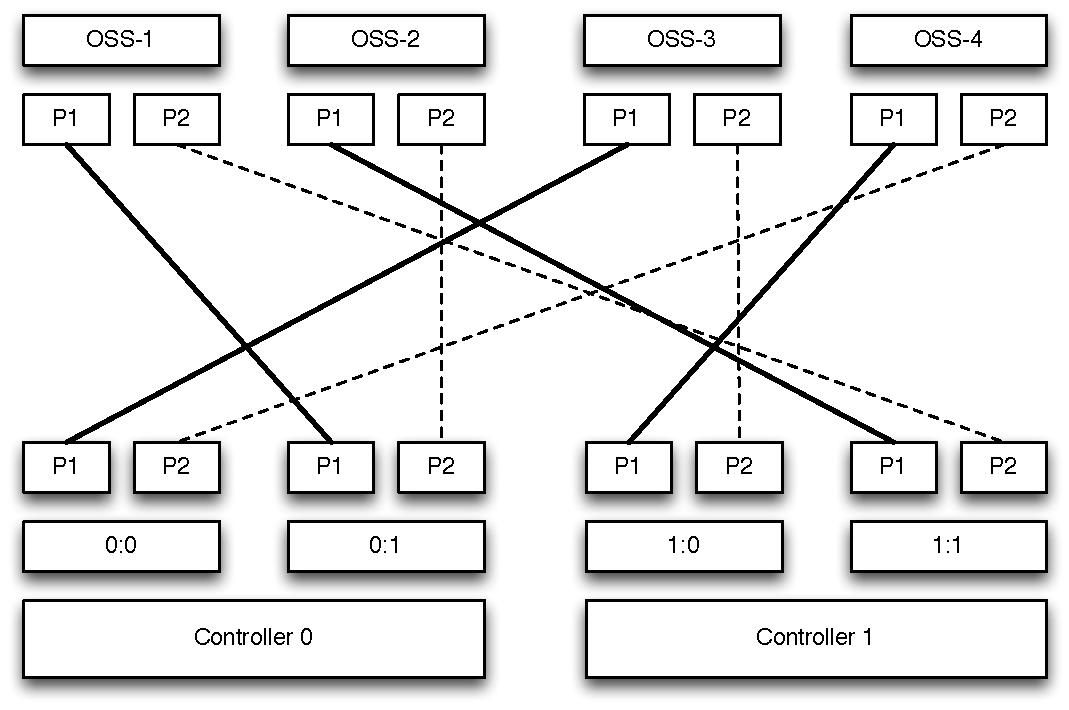
\includegraphics[width=4in]{figs/sfa10k}
\caption{DDN SFA10K Hardware Diagram}
\end{figure}


The supporting infrastructure nodes are summarized in the following table:

\begin{table}[H]
\centering
    \begin{tabular}{ll}
    \toprule
    Node & Role \\
    \midrule
    tick-mds1 & Ceph monitor node \\
    spoon46 & Ceph MDS node \\
    tick-oss[1-4] & Ceph OSD servers \\
    spoon28-31, spoon37-41 & Ceph client nodes \\
    \bottomrule

    \end{tabular}

\end{table}

The hosts are running Redhat 6.3 with 3.5.1 kernel (rhl-ceph image), Glibc 2.12
with syncfs support, locally patched. The Ceph version is 0.55 release in the
initial test, then upgraded to 0.64 and 0.67RC for second round of test. For a
complete a list of hosts that are running ceph images, you can do:

\begin{Verbatim}
grep "rhel6-ceph" /etc/gedi/MAC.info
\end{Verbatim}


\section{Baseline Performance}


\subsection*{Block I/O}
We first establish the baseline performance by measuring block I/O performance.
At the block level, with LUN configured as RAID6 8+2, we have the following
results:

\begin{table}[htb]
\centering
\begin{tabular}{ll}
    \toprule
    SAS single LUN sequential read & ~1.4 GB/s \\
    SATA single LUN sequential read & ~955 MB/s \\[0.5em]
    Single host with 4 SAS LUNs & ~ 2.8 GB/s \\
    Single host with 7 SATA LUNs & ~ 2.6 GB/s \\
    \bottomrule
\end{tabular}

\end{table}

Single host refers to one of 4 tick-oss nodes, which drives the entire SSU.
Overall, the entire SSU performance can perform at 11GB/s, comparing to
theoretical maximum of 12GB/s.


\subsection*{IP over IB}

Note that we are using IP over IB for networking, since Ceph doesn't have
native IB support\footnote{Inktank is developing rsocket alternative to better take
advantage of IB fabric}.
A single host with IP over IB (QDR) can perform at 2.7 GB per second with
Mellanox recommended tuning applied. With all 4 hosts (OSD servers), we expect
the aggregate throughput is in the neighborhood of 10GB/s.

Unfortunately there was not enough time to do more detailed analysis of network
bisection bandwidth. Later, we will see RADOS is performing a
maximum of 5 to 6 GB per seconds driven by 4 hosts.  So, this test shows that we
have enough network bandwidth, i.e., IP over IB is not a bottleneck in this
case.




\section{The Starting Point of System Tuning}

Base upon past experience and further experimentation, we started out on the
following set of tuning parameters:

\begin{table}[htb]
\centering
\begin{tabular}{ll}
    \toprule
    \verb!nr_requests! & 2048 \\
    \verb!read_ahead_kb! & 4096 \\
    \verb!scheduler! & deadline \\
    \bottomrule
\end{tabular}

\end{table}



\section{XFS Performance}

As we plan to use XFS file system as the backend local file system for Ceph, we
examine XFS against SFA10K to acquire a set of sensible configuration parameters
for optimized performance. We sampled a selected set of parameters (block size,
queue depth, request size, sequential read and write), and this is the
configurations we selected: mount with \verb!nobarrier,noatim,inode64! options.
The \verb!inode64! option had a notable improvement on sequential write (around
20\%).

\begin{figure}[htb]
\centering
%% -- 1st figure
\begin{minipage}[t]{0.5\linewidth}
\centering
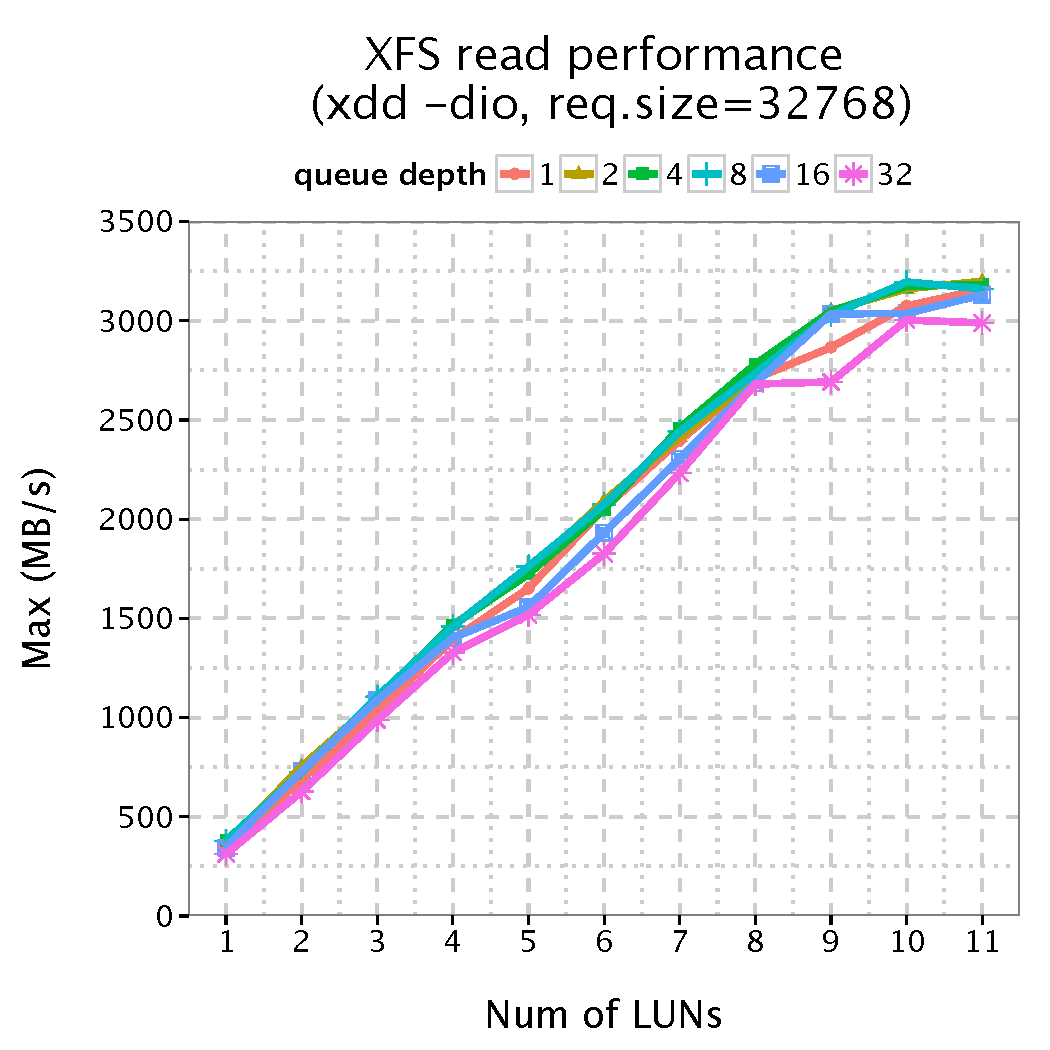
\includegraphics[width=3in]{data/xdd-read}
\caption{XFS read scaling on \# of devices}
\label{fig:xfs-read}
\end{minipage}%
\begin{minipage}[t]{0.5\linewidth}
\centering
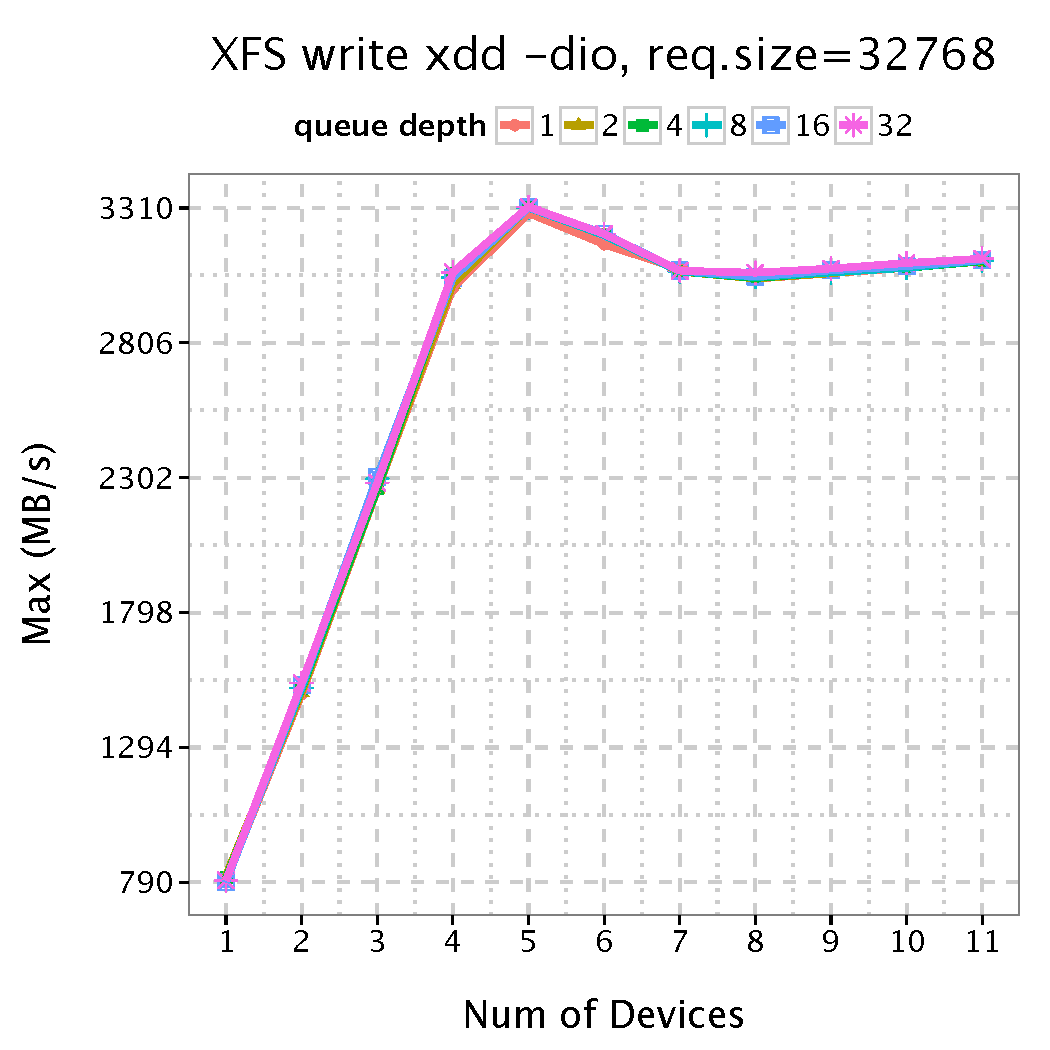
\includegraphics[width=3in]{data/xdd-write}
\caption{XFS write scaling on \# of devices}
\label{fig:xfs-write}
\end{minipage}%
\end{figure}

The read and write result are summarized in Figure~\ref{fig:xfs-read}
and Figure~\ref{fig:xfs-write}. These scaling test on the number of devices
indicates that XFS can get to peak read performance with 5 SATA LUNs, then there
is a bit of degradation from there. The parameter space explored regarding to
the queue depth doesn't seem to make any obvious difference on the performance
though.




\section{Ceph RADOS Scaling: Initial Test}

RADOS is Ceph object store, a foundational component for CephFS file
system. There are three types of scaling tests we are interested at RADOS layer:

\begin{itemize}
  \item scaling on the number of servers
  \item scaling on the number of clients
  \item scaling on the number of OSDs
\end{itemize}

Our system setup poses some limitation on the scalability test we want to
perform. In particular, we currently have 4 OSS server, 8 clients, and 11 OSD
per clients. So the scaling test will be within these constraints. 

An open source tool developed by Inktank called RADOS bench was do perform
initial performance analysis of the underlying RADOS layer.  RADOS Bench simply
writes out objects to the underlying object storage as fast as possible, and
then later reads those objects in the same order as they were written.

We've observed that using more than one client processes and lots of concurrent
operations is important when performing these tests.  8 Client processes are
used with 32 concurrent 4MB Objects in flight each, and a pool is created for
each RADOS bench process to ensure that object reads come from independent pools
(RADOS bench is not smart enough to ensure that objects are not read by multiple
processes and thus possibly cached).  A sync and flush is performed on every
node before every test to ensure no data or metadata is in cache.  All tests
were run with 1X replication.  Unfortunately at this time only XFS was present
and usable for the underlying OSDs so BTRFS and EXT4 file systems were not
tested at this time.


\subsection{Scaling on number of OSDs}

In the following test, a single Ceph host drives $n$ number of OSDs, where $n$
increases from 1 to 11. The result is illustrated in Figure~\ref{fig:osd-scale}.
We ran the test against a single client with 4 concurrent process. In this test
case, we observe that Ceph OSS exhibits near linear scalability up to 9
OSDs, and still have room to grow at 11 OSDs. This suggests that we have not reached the
saturation point yet. It requires provisioning of more OSDs at SFA10K backend.


\begin{figure}[H]
\centering
%% -- 1st figure
\begin{minipage}[t]{0.5\linewidth}
\centering
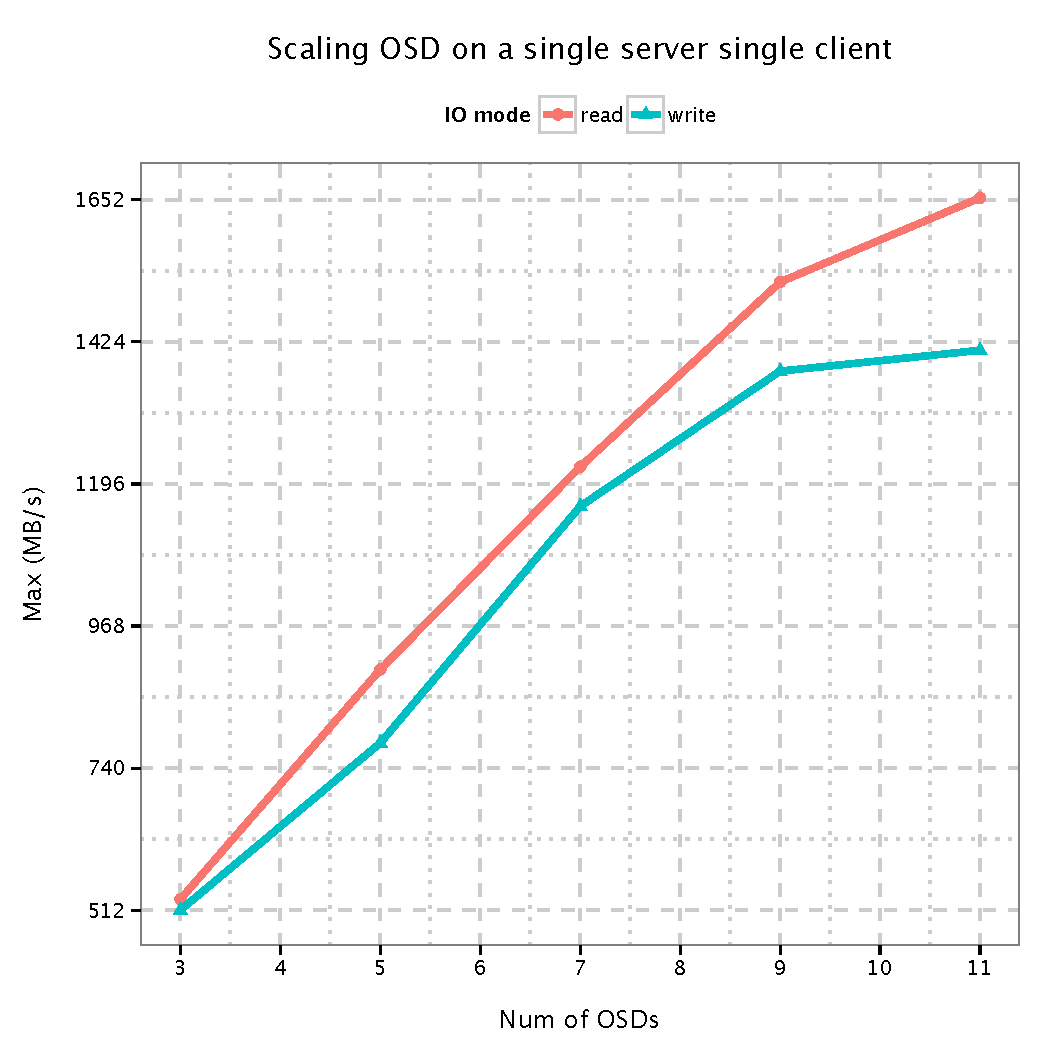
\includegraphics[width=3in]{data/rados_osd}
\caption{RADOS scaling on \# of OSDs}
\label{fig:osd-scale}
\end{minipage}%
\begin{minipage}[t]{0.5\linewidth}
\centering
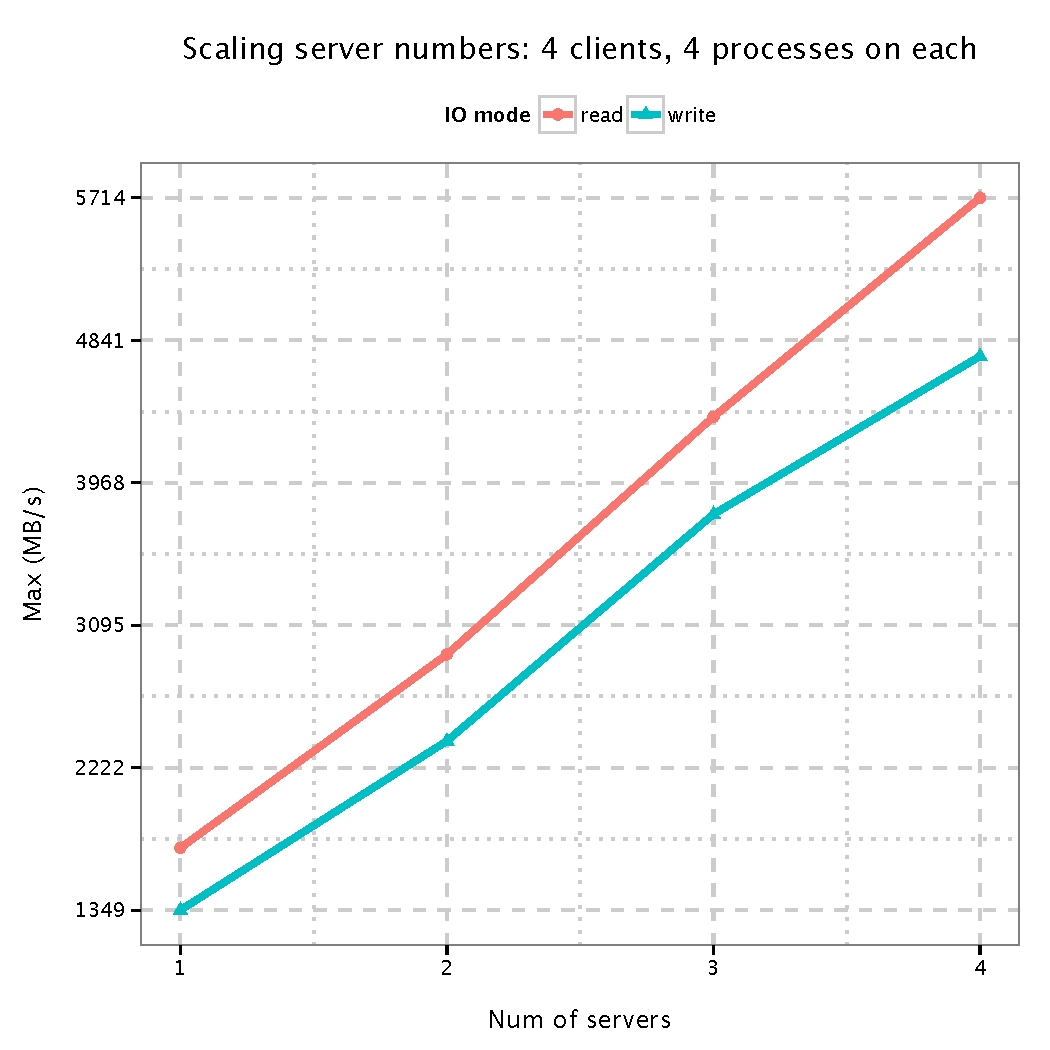
\includegraphics[width=3in]{data/rados_server}
\caption{RADOS scaling on \# of servers}
\label{fig:oss-scale}
\end{minipage}%
\end{figure}

\subsection{Scaling on number of servers}

In this test, we exercise OSS number from 1 to 4, driven by 4 clients with 4
concurrent process for each client. Each addition of OSS adds 11 more OSDs into
the play. We observe that Ceph exhibits linear scaling property with regard to
number of servers as well, at least in the given set of servers. However, the peak
performance we are seeing is about the half of what are expecting from SFA10K.
For the write, the reason behind it is attributed to the way Ceph perform
journaling: Ceph doesn't support the meta-data only journaling, therefore every
write is equivalent of a double-write: once to the data device, once to the
journaling device. It effectively cut the system bandwidth in half. That said,
it doesn't explain the read performance - though it is better than write, but is
still far from the theoretical maximum.

\section{Ceph File System Performance: Initial Test}

We use synthetic IOR benchmark suite for file system level test. The particular
parameter setup is show in Table \ref{tbl:ior}. Each client node has 6 GB
physical memory, the block size is set so as to mitigate the cache effect. In
addition, the test harness program will issue the following command at the
beginning of each test:




\begin{table}[tb]
\centering
\begin{tabular}{p{1.5in} | p{3in}}
    \toprule
    IOR parameter & Note \\ \midrule
    \verb!-F! & file per process \\ \midrule
    \verb!-a POSIX! & use POSIX API \\ \midrule
    \verb!-w -r -C! & do both write and read test, \verb!-C! is to change task
        ordering for read back so it won't read from the write cache. \\ \midrule
    \verb!-i 3 -d 5! & 3 iterations and delay 5 seconds betewen iterations \\
    \midrule  
    \verb!-e! & perform \verb!fsync()! upon POSIX write close \\ \midrule
    \verb!-b 8g or 16g! & the block size \\ \midrule
    \verb!-t 4k to 4m! & the transfer size \\ \midrule
    \verb!-o file! & mandatory test file  \\    
    \bottomrule
\end{tabular}
\caption{IOR parameter setup}
\label{tbl:ior}
\end{table}


\begin{Verbatim}
# sync
# echo 3 | tee /proc/sys/vm/drop_caches
\end{Verbatim}


Here, 0 is the default value of \verb!drop_cahces!; 1 is to free pagecaches, 2
is to free dentries and inodes, 3 is to free pagecache, dentries, and inodes.


Our first round of test was less than ideal as we encountered various issue. For
the sake of completeness, we still first summarized the results, then discuss
the further tuning efforts and improvements.

The full permutation of IOR parameters are not explored due to IO errors we ran
into. We were, however, able to record results in two extreme case as far as
transfer size is concerned: 4KB and 4MB, using the same number of OSS servers
(4) and same block size (8GB), the results are illustrated in Figure
\ref{fig:ior4k} and \ref{fig:ior4m}, we make the following observations:


\begin{figure}[H]
\centering
%% -- 1st figure
\begin{minipage}[t]{0.5\linewidth}
\centering
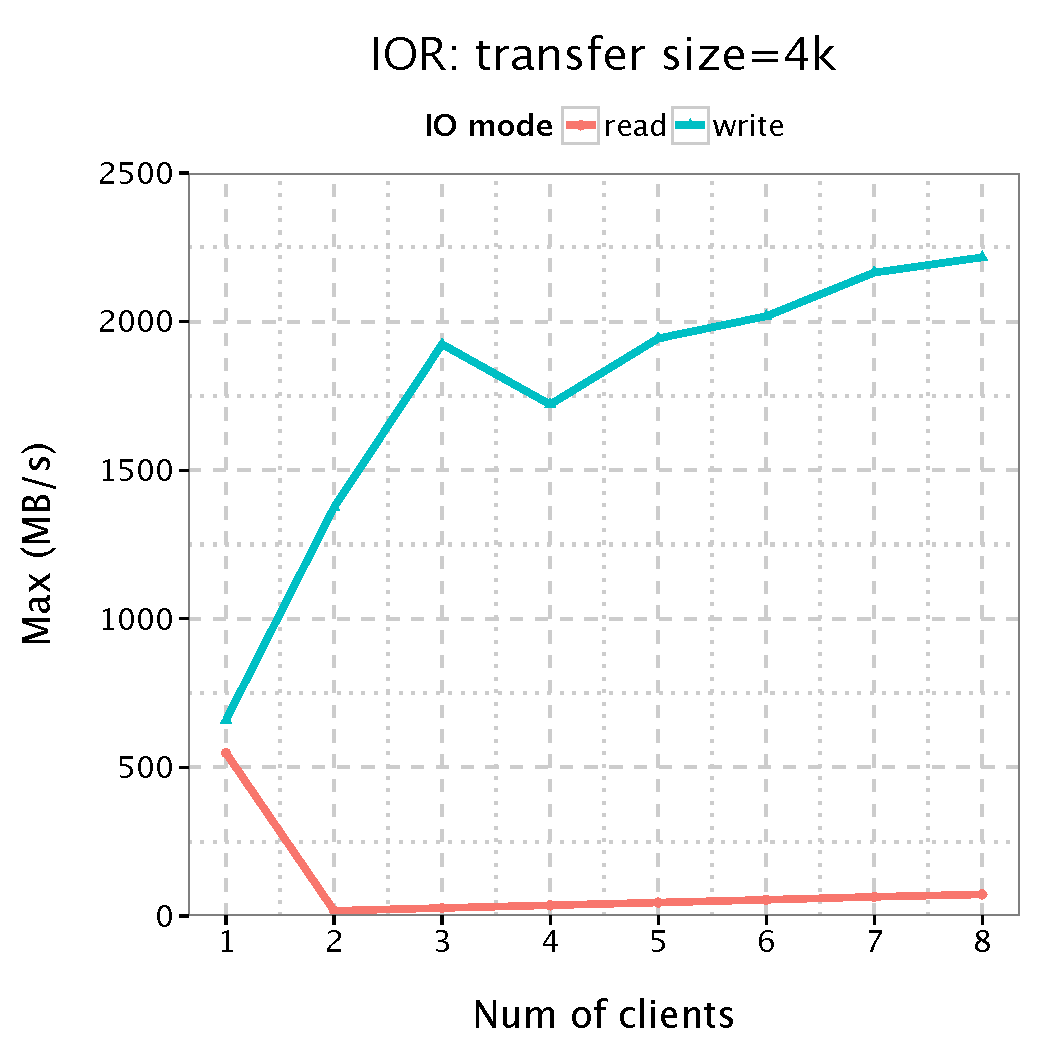
\includegraphics[width=3in]{data/ior_4k}
\caption{IOR tests: 4k transfer size}
\label{fig:ior4k}
\end{minipage}%
\begin{minipage}[t]{0.5\linewidth}
\centering
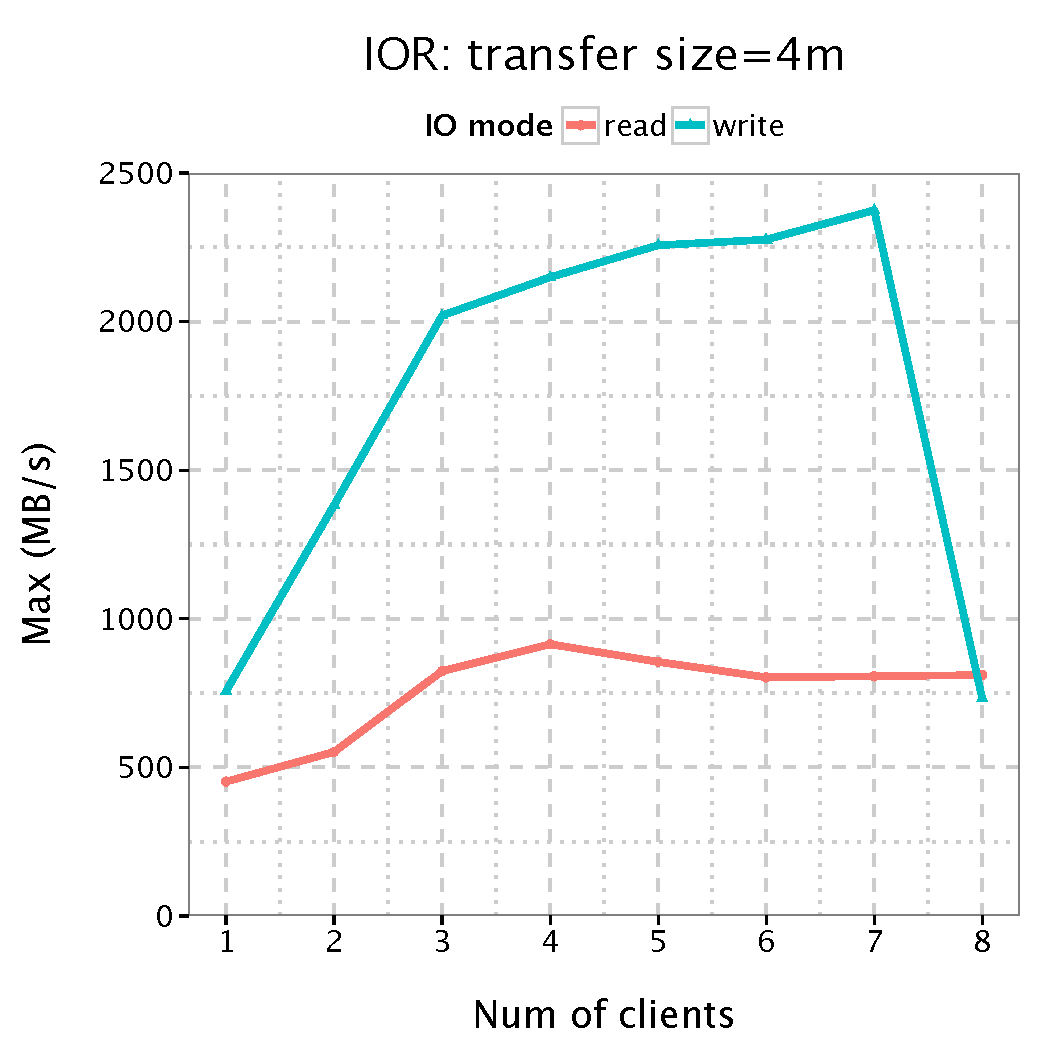
\includegraphics[width=3in]{data/ior_4m}
\caption{IOR tests: 4m transfer size}
\label{fig:ior4m}
\end{minipage}%
\end{figure}


\begin{itemize}
  \item The small read performance is almost an anomaly - we need to
  investigate why it is so low compare to write.
  \item The large read performance is almost half of the write performance,
  which is the opposite of RADOS level. 
  \item The write performance is cut in half compare to what we can obtain from
  RADOS benchmark. And number of clients reaches 8, there is a significant
  performance drop as well. 
\end{itemize}


%\begin{figure}[htb]
%\centering
%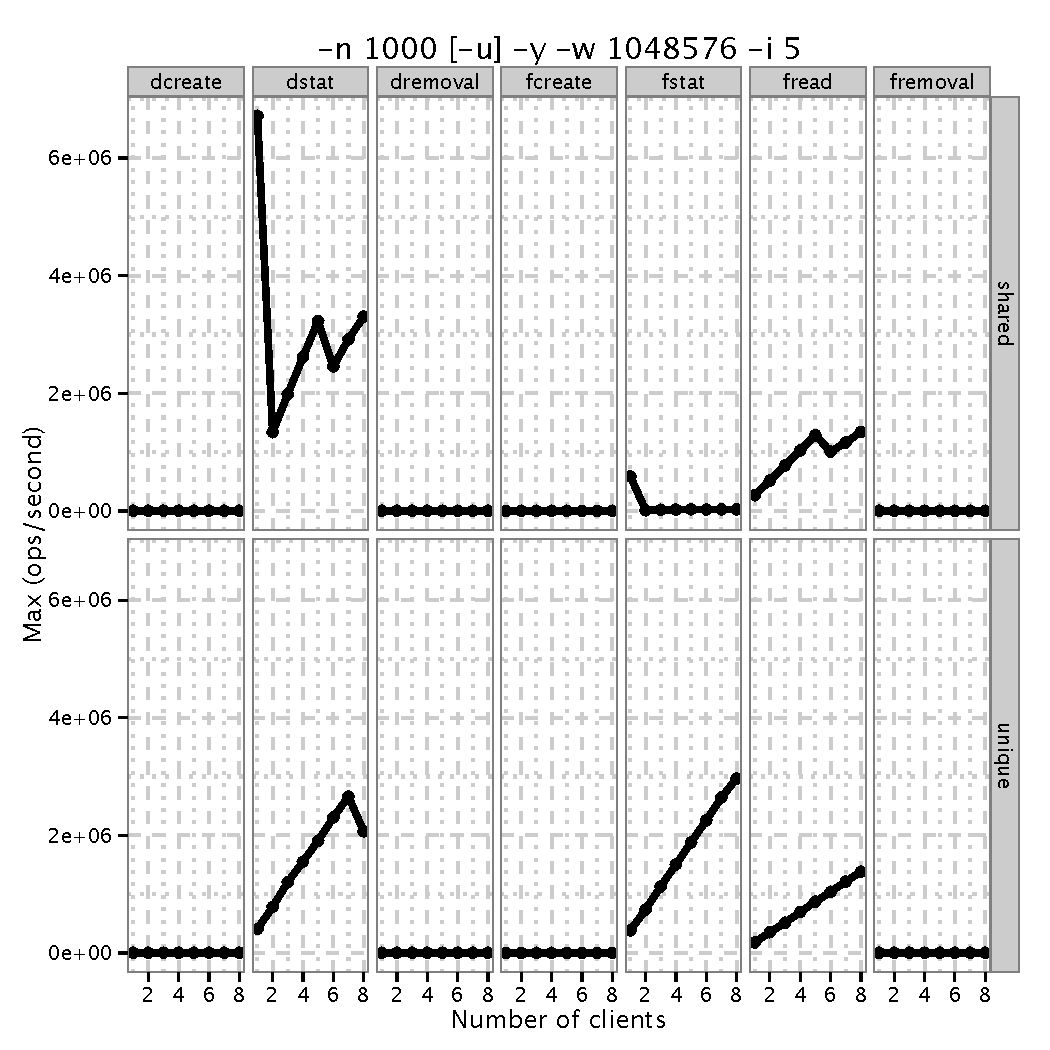
\includegraphics[width=5in]{data/mdtest}
%\caption{mdtest of single MDS}
%\label{fig:mdtest1c}
%\end{figure}

We will describe the efforts and results on performance improvement in the
following sections.

\section{Improving RADOS Performance}

\begin{figure}[h]
\centering
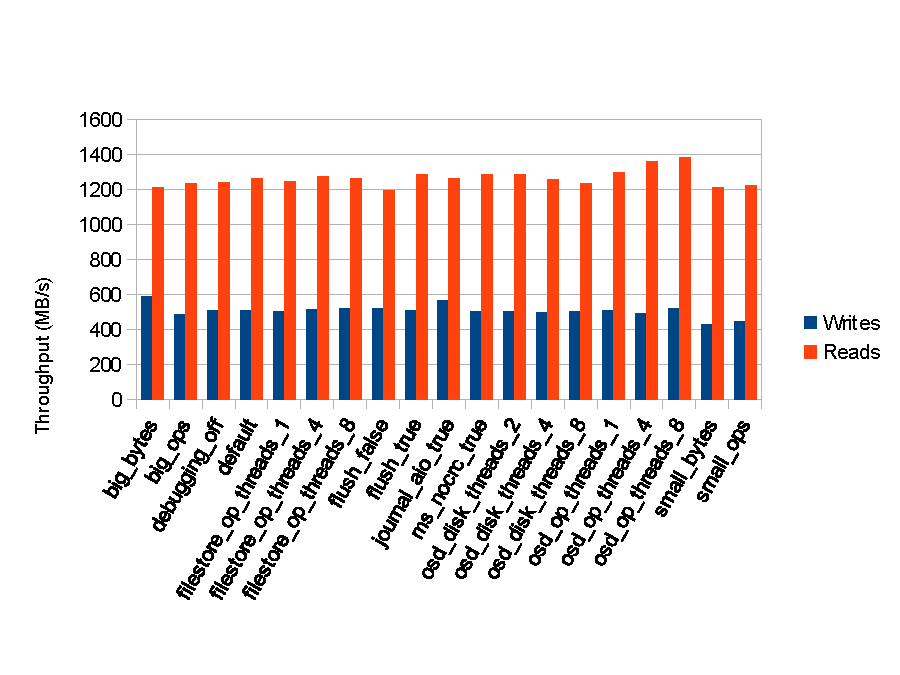
\includegraphics[width=5in]{parametric}
\caption{Evaluating parameter impact through sweeping test}
\label{fig:parametric}
\end{figure}


After the initial test results were found, various combinations of tweaks were
attempted including changing the number of filestore op threads, putting all
of the journals on the same disks as the data, doubling the OSD count, and
upgrading Ceph to a development version which reduces the seek overhead caused
by \texttt{pginfo} and \texttt{pglog} updates on XFS (These enhancements are
now included as of the Ceph Cuttlefish release).  The two biggest improvements
resulted from disabling CRC32c checksums and increasing the OSD count on the
server.  With these changes, we are seeing better results.

A script written by Inktank for internal Ceph testing was used to perform
parametric sweeps over Ceph configuration parameters to examine how different
tuning options affect performance on the DDN platform. The result of this
parameter probing is illustrated in Figure~\ref{fig:parametric}. 

As a result of this testing, performance was again improved slightly by
increasing the size of various Ceph buffers and queues, enabling aio journals,
and increasing the number of OSD op threads.


\subsection{Disable Cache Mirroring on DDN}


Despite the excellent write throughput we saw during the individual server
tests, throughput did not scale.  A significant amount of time was spent
investigating this phenomena. Ultimately, we were able to replicate this finding
when running concurrent disk throughput tests directly on the servers without
Ceph involved. The 2nd RAID processor on each DDN controller would max out when
3 or more LUNs were written concurrently. It turns out the root of the problem
is attributed to a regression on DDN firmware update - in particular, the cache
mirroring is not behaving as it should be. 


\begin{figure}[htb]
\centering
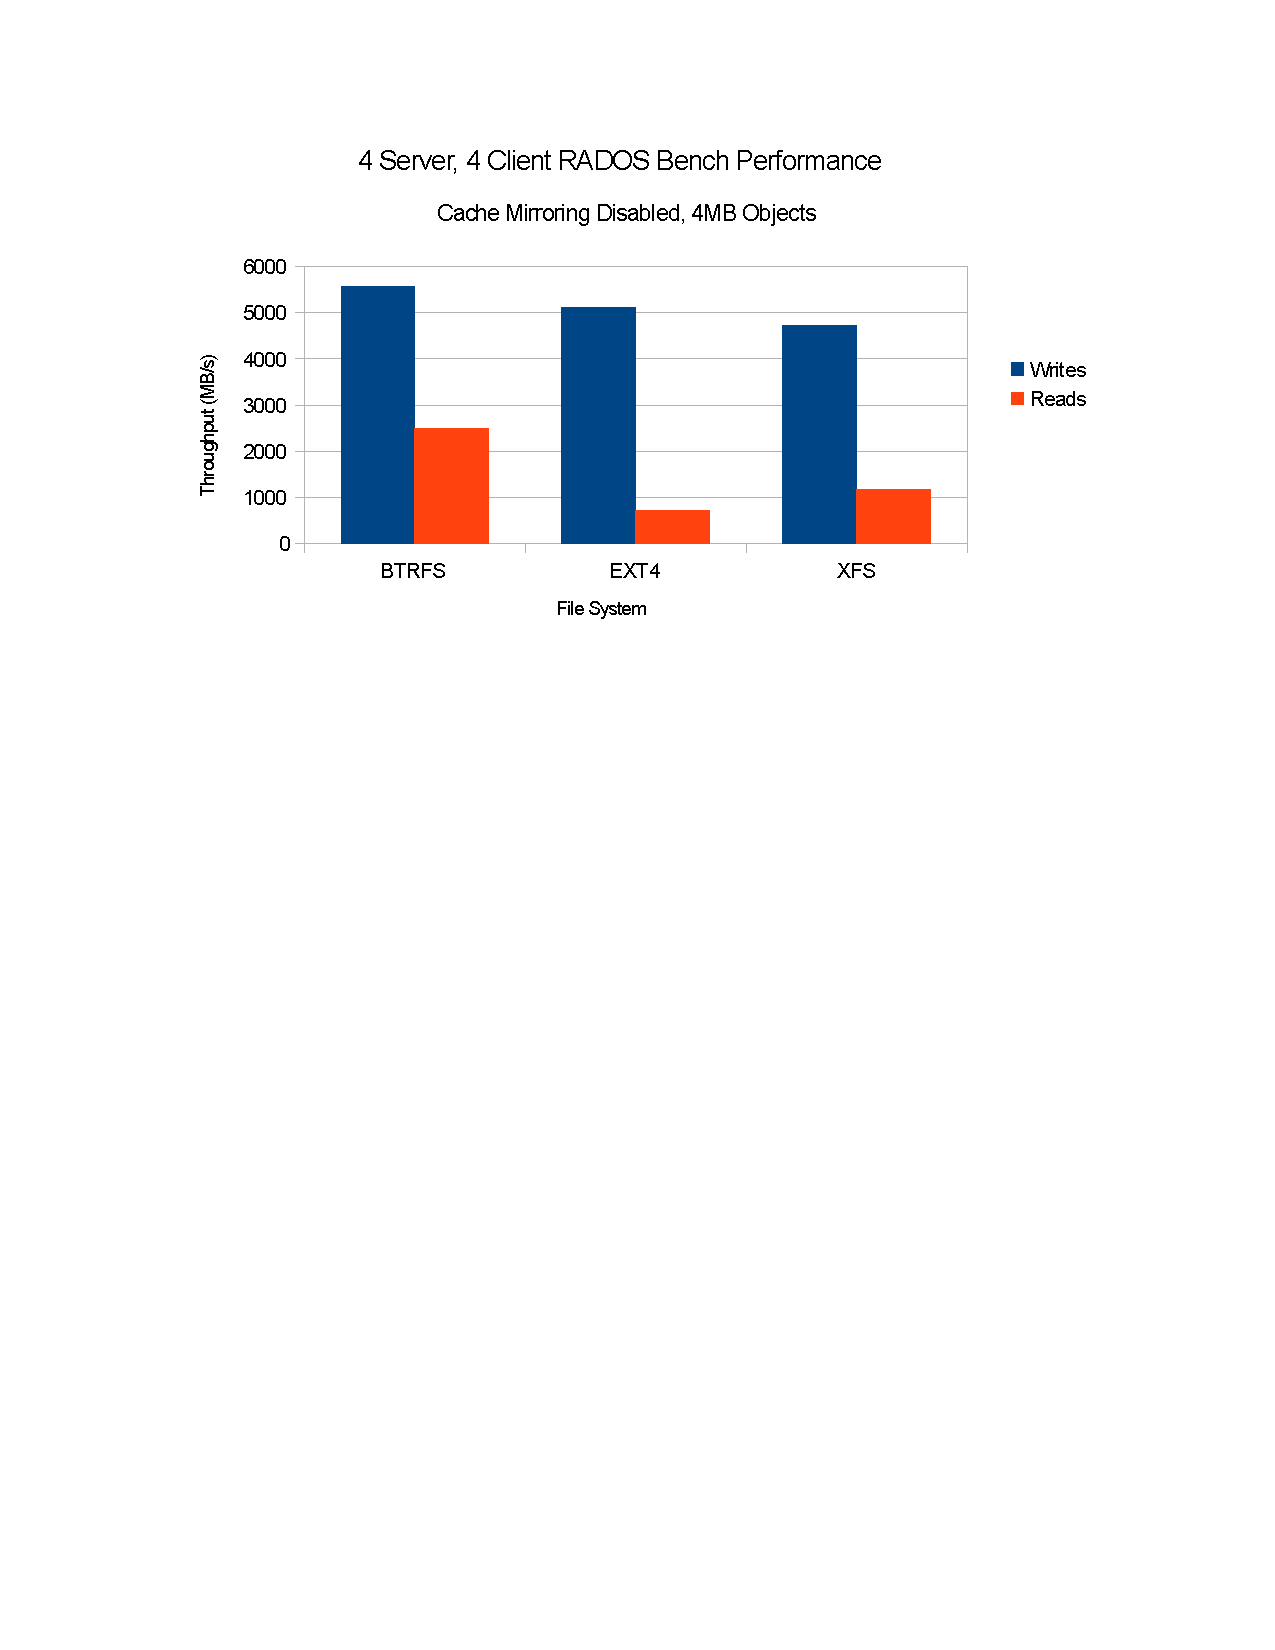
\includegraphics[width=4in]{rados-after-ddn}
\caption{Evaluating RADOS bench after disabling cache mirroring}
\label{fig:rados-ddn-mirror-disabled}
\end{figure}


With cache mirroring disabled write performance when using all 4 servers
improved dramatically, as illustrated in
Figure~\ref{fig:rados-ddn-mirror-disabled}. With BTRFS for example, we hit over
5.5GB/s from the clients.  When accounting for journal writes, that is over
11GB/s to the disks and very close to what the DDN chassis is capable of doing. 
Unfortunately, read performance did not scale as well.


\subsection{Disable TCP autotuning}

During these tests, a trend that previously had been seen became more apparent.
During reads, there were periods of high performance followed by periods of low
performance or outright stalls that could last for up to 20 seconds at a time. 
After several hours of diagnostics, Inktank observed that outstanding operations
on the clients were not being shown as outstanding on the OSDs.  This appeared
to be very similar to a problem Jim Schutt at Sandia National labs encountered
with TCP autotuning in the Linux Kernel.
\footnote{\url{http://marc.info/?l=ceph-devel&m=133009796706284&w=2}}.
TCP auto tuning enables TCP window scaling by default and automatically adjust
the TCP receive window for each connection based on link conditions such as
bandwidth delay product. We have observed this will make a notable improvement
on Ceph read performance, as the results shown in
Figure~\ref{fig:rados-tcp-auto-disabled}.


Luckily, the fix was fairly straight forward by issuing the following command on all nodes:

\begin{Verbatim}
     echo 0 | sudo tee /proc/sys/net/ipv4/tcp_moderate_rcvbuf
\end{Verbatim}

Recent versions of Ceph work around this issue by manually controlling the TCP
buffer size.  The testing at ORNL directly influenced and motivated the creation
of this feature!

\begin{figure}[htb]
\centering
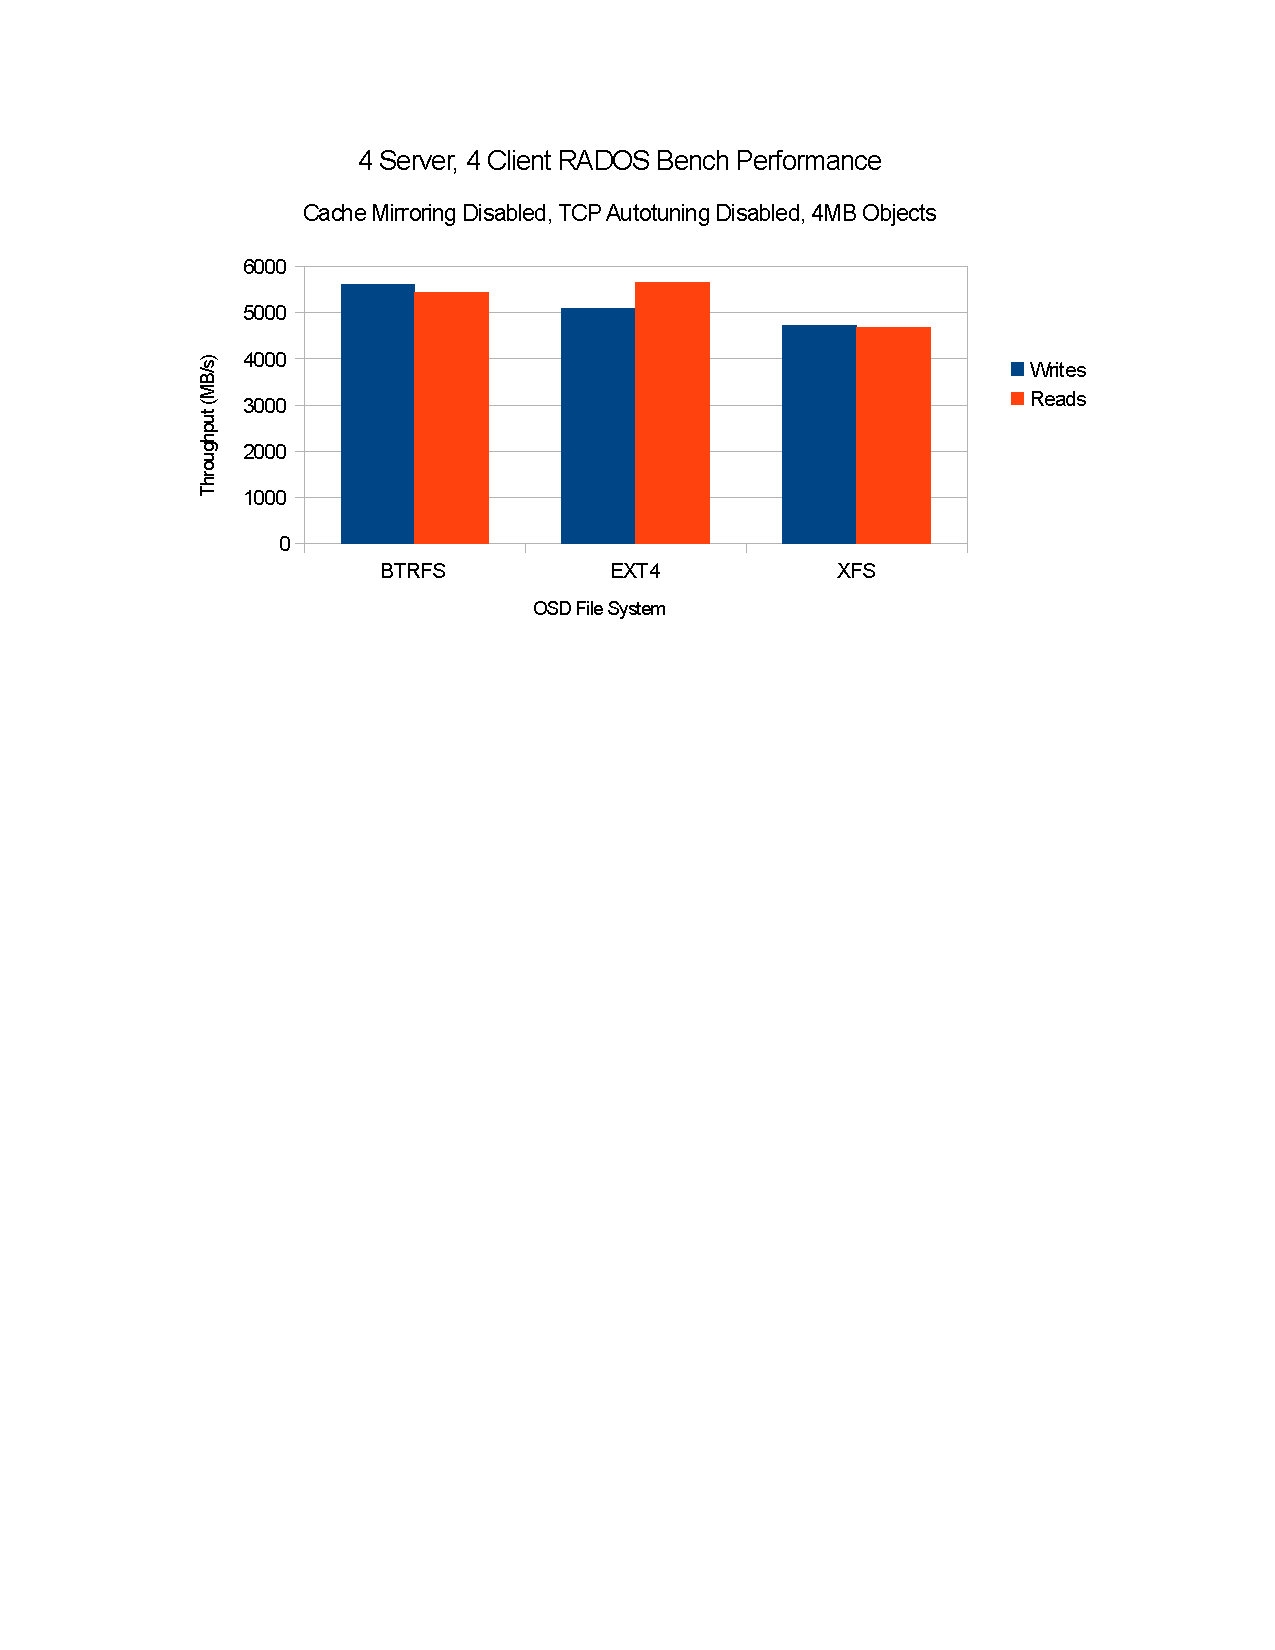
\includegraphics[width=4.0in]{rados-after-ddn-tcptune}
\caption{Evaluating RADOS bench after TCP auto tuning disabled}
\label{fig:rados-tcp-auto-disabled}
\end{figure}



%\begin{figure}[htb]
%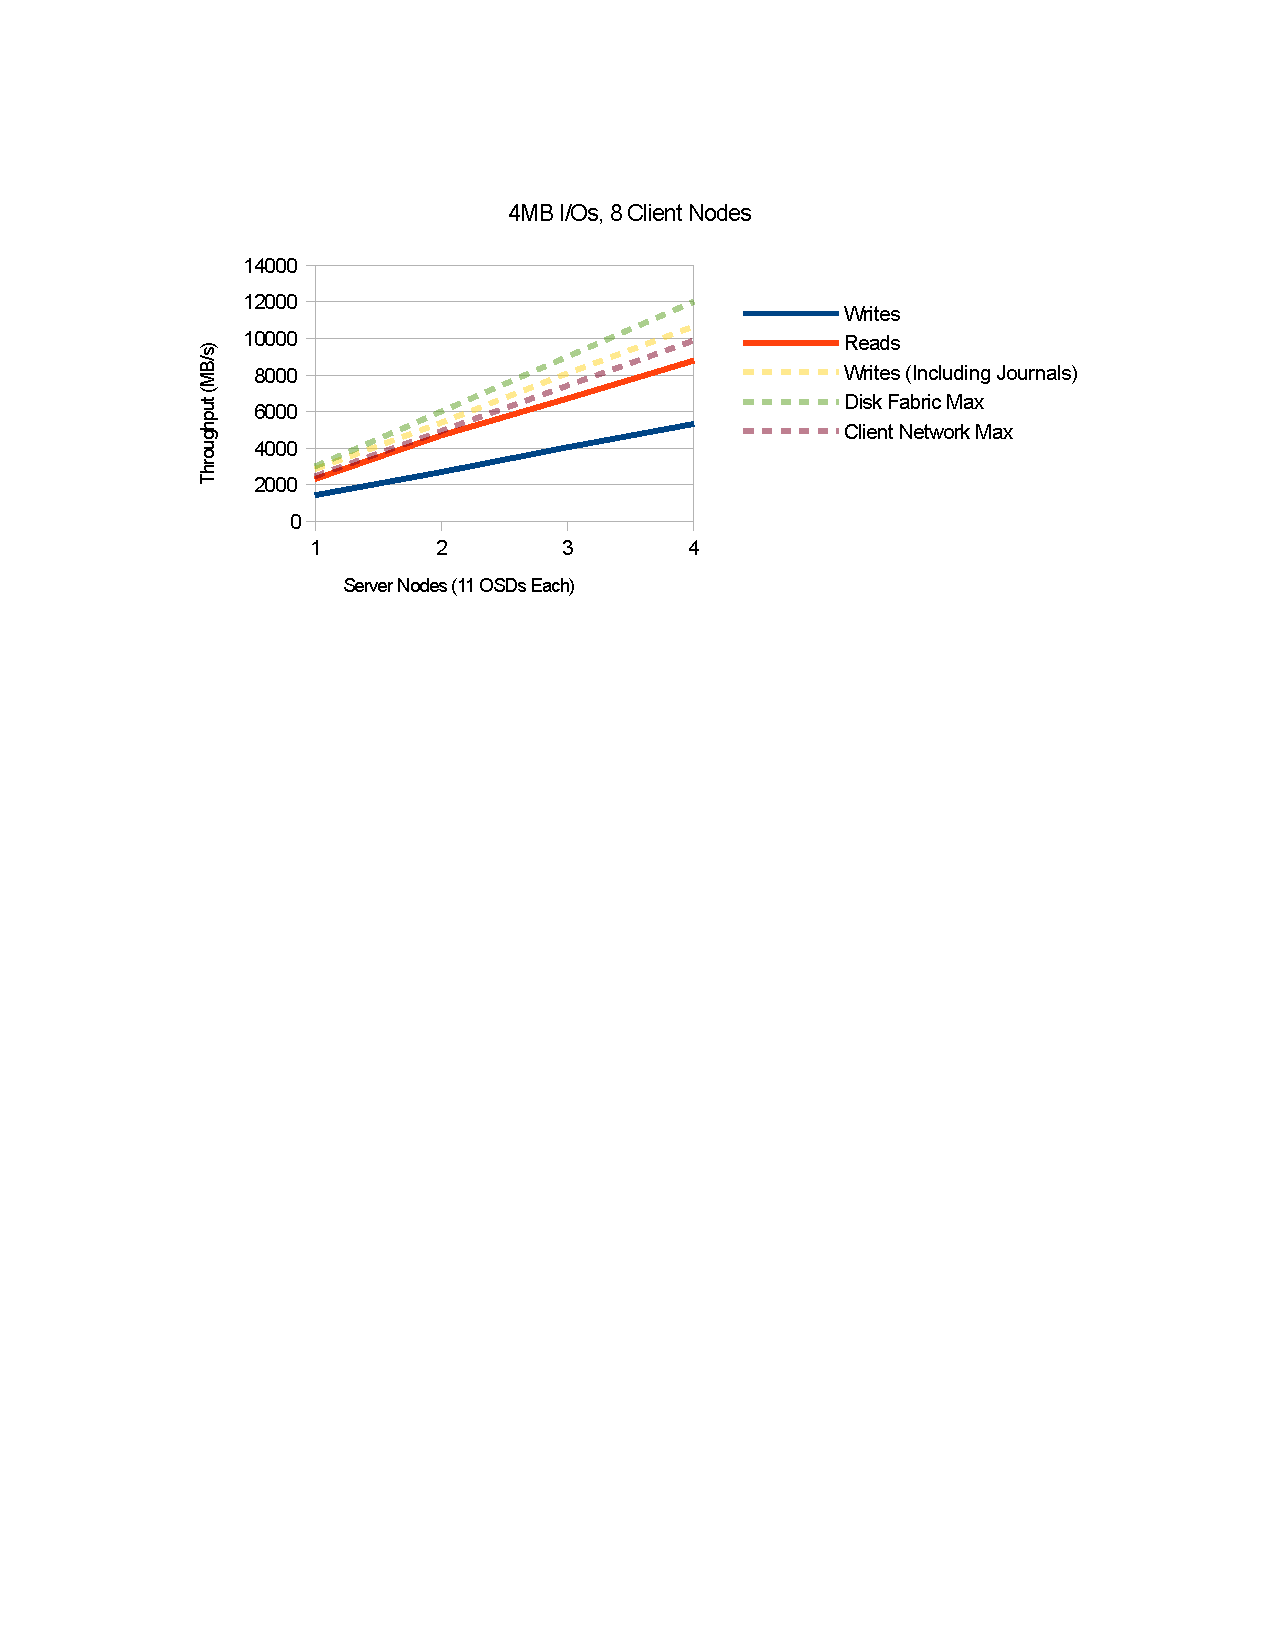
\includegraphics[width=5in]{rados-064-oss}
%\end{figure}

\subsection{Repeating RADOS Scaling Test}

We now repeated previous RADOS scaling test with these improvements in place.
The first test was done on a single node with RADOS bench to see how close the
underlying object store could get to the node hardware limitations as the number
of OSDs/LUNs used on the node increase. Note all the tests performed are against
XFS formatted storage.

\begin{figure}[htb]
\centering
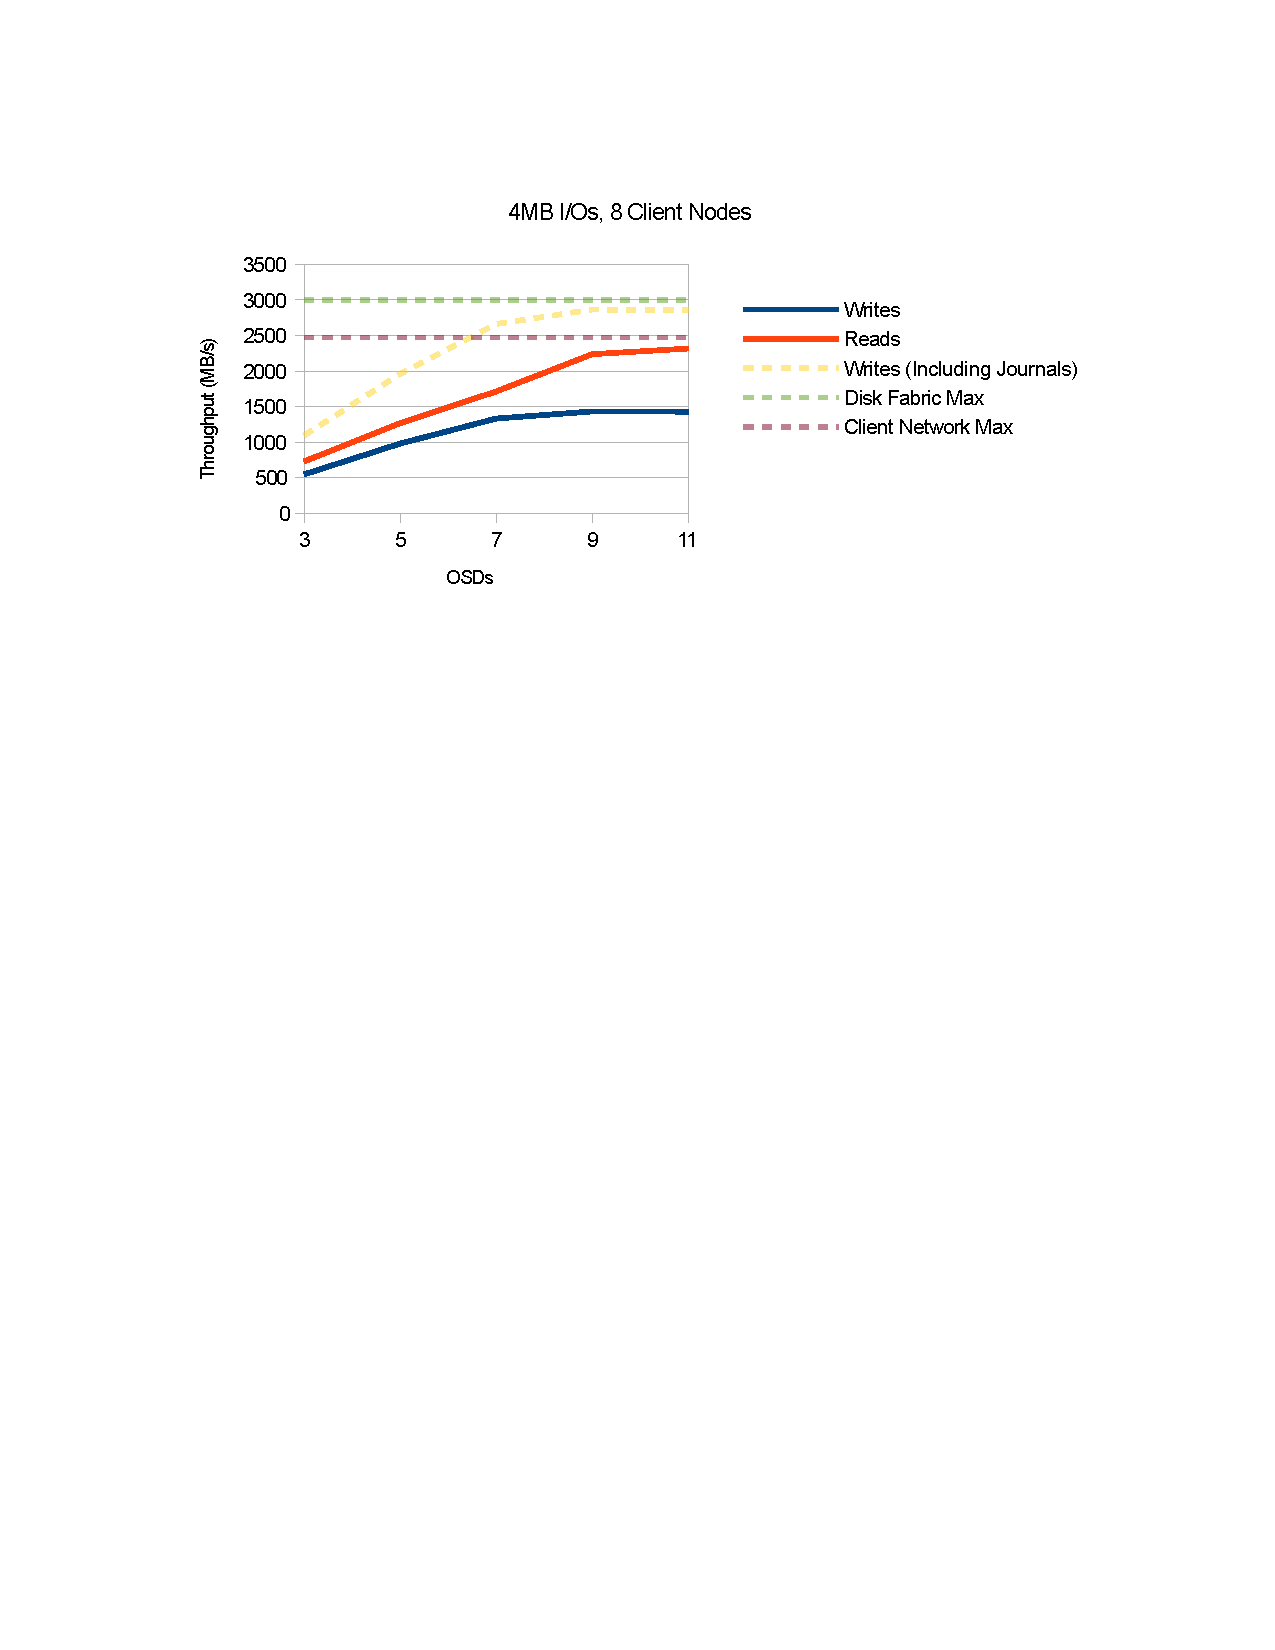
\includegraphics[width=5in]{rados-064-osd}
\caption{RADOS Bench Scaling on \# of OSD, Ceph 0.64, 4MB IO, 8 Client Nodes}
\label{fig:rados-064-osd}
\end{figure}

In the single server case as shown in Figure~\ref{fig:rados-064-osd},
performance gets very close to the hardware limits at roughly 9 OSDs per server
and then mostly levels out.

We also repeated tests looking at RADOS Bench performance as the
number of OSD server nodes increases. The result is summarized in
Figure~\ref{fig:rados-064-oss}. As the number of nodes increases, performance
scales nearly linearly for both reads and writes.


\begin{figure}[htb]
\centering
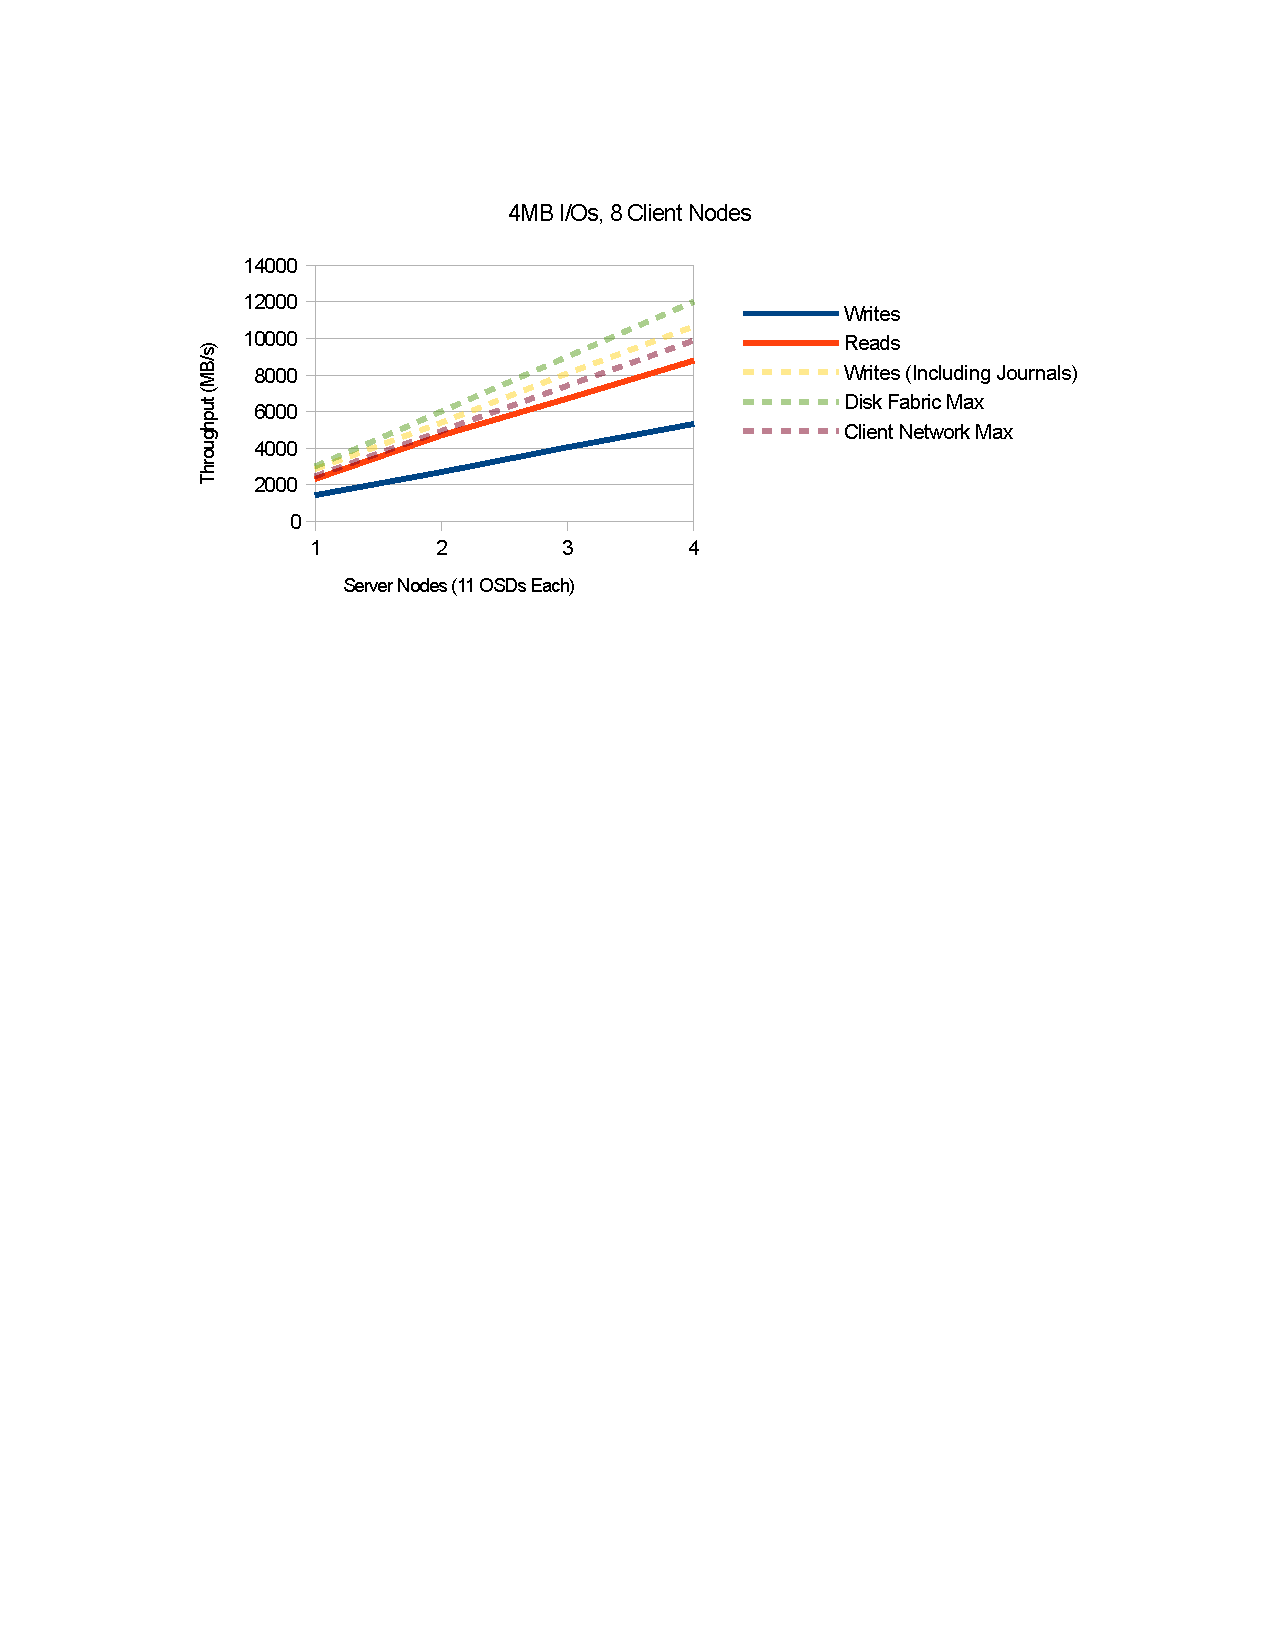
\includegraphics[width=5in]{rados-064-oss}
\caption{RADOS Bench Scaling on \# of Server, Ceph 0.64, 4MB IO, 8 Client Nodes}
\label{fig:rados-064-oss}
\end{figure}



\section{Improving Ceph File System Performance}

The initial stability issues we encountered are fixed by moving Ceph version
from 0.48/0.55 to 0.64, latest stable at the time. Now IOR test can proceed to
finish even during long runs. It is another sign of showing how much Ceph
development is in flux.

Another fix comes the way we create the pool: the default data pool being used
by previous CephFS cluster are set to 2x replication, which can potentially
halve the write performance. Even with these changes in place, Inktank still
reproduced the less-than-ideal write performance and very poor read
performance as observed by ORNL.  Further, by increasing the number of IOR
processes per client node, read performance actually degraded further
indicating some kind of contention either on the clients or on the OSD
servers.


\subsection{Disabling Client CRC32}

ORNL at this point was able to both make more client nodes available and also
install a profiling tool called \verb!perf! that is extremely useful for
profiling both kernel and user space code.  Profiling with \verb!perf! showed
high CPU utilization on the client due to crc32c processing in the Ceph kernel
client.  Luckily crc32 checksums can be disabled by changing the CephFS mount
options:

\begin{Verbatim}
mount -t ceph 10.37.248.43:6789:/ /mnt/ceph -o name=admin,nocrc
\end{Verbatim}


With client CRC32 disabled, we repeated the IOR test and the results are showin
in Figure~\ref{fig:ior-no-client-crc32}. 

\begin{figure}[htb]
\centering
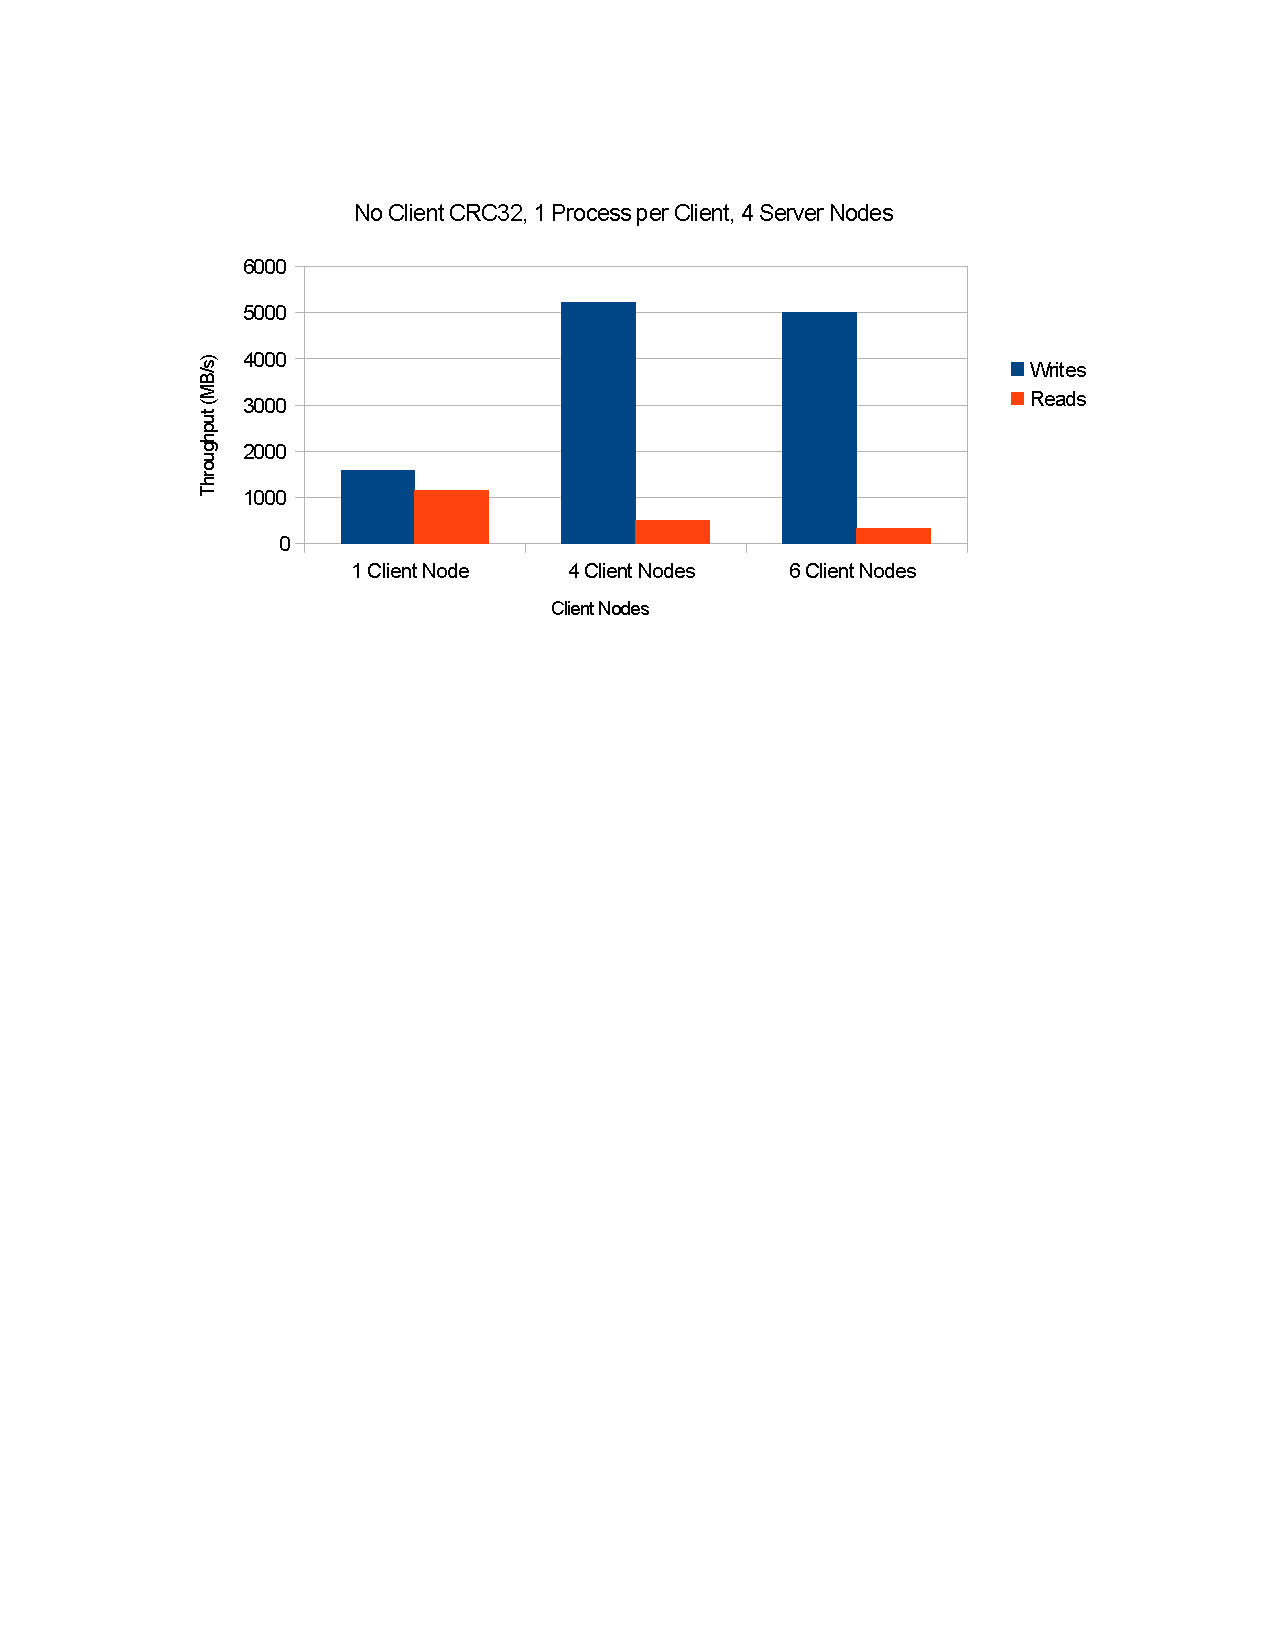
\includegraphics[width=4in]{ior-client-no-crc32}
\caption{IOR test with no client side CRC32}
\label{fig:ior-no-client-crc32}
\end{figure}

We observed that IOR write throughput increased dramatically and is now very
close to the throughput we were able to achieve with RADOS Bench, but reads
continued to be slow, and continued to inversely scale with the number of client
processes.  Please note that since these tests were performed, Inktank has
implemented SSE4 based CRC32 code for Intel CPUs.  While any kernel based CRC32
processing should have already been using SSE4 instructions on Intel CPUs, this
will allow any user land Ceph processes to process CRC32 checksums with
significantly less overhead.

\subsection{Improving IOR Read Performance}

Deeper analysis with perf showed that there was heavy lock contention during
parallel compaction in the Linux kernel memory manager.  This behavior was first
observed roughly in the kernel 3.5 time frame which happens to be the kernel
that ORNL had installed on the test systems.\footnote{For more information,
please refer to \url{http://lwn.net/Articles/517082/} and
\url{https://patchwork.kernel.org/patch/1338691/}.}

ORNL installed kernel 3.9 on all of the test systems and Inktank performed a
RADOS bench test to verify that there was no degradation vs previous tests.  The
results were extremely positive.


\begin{figure}[htb]
\centering
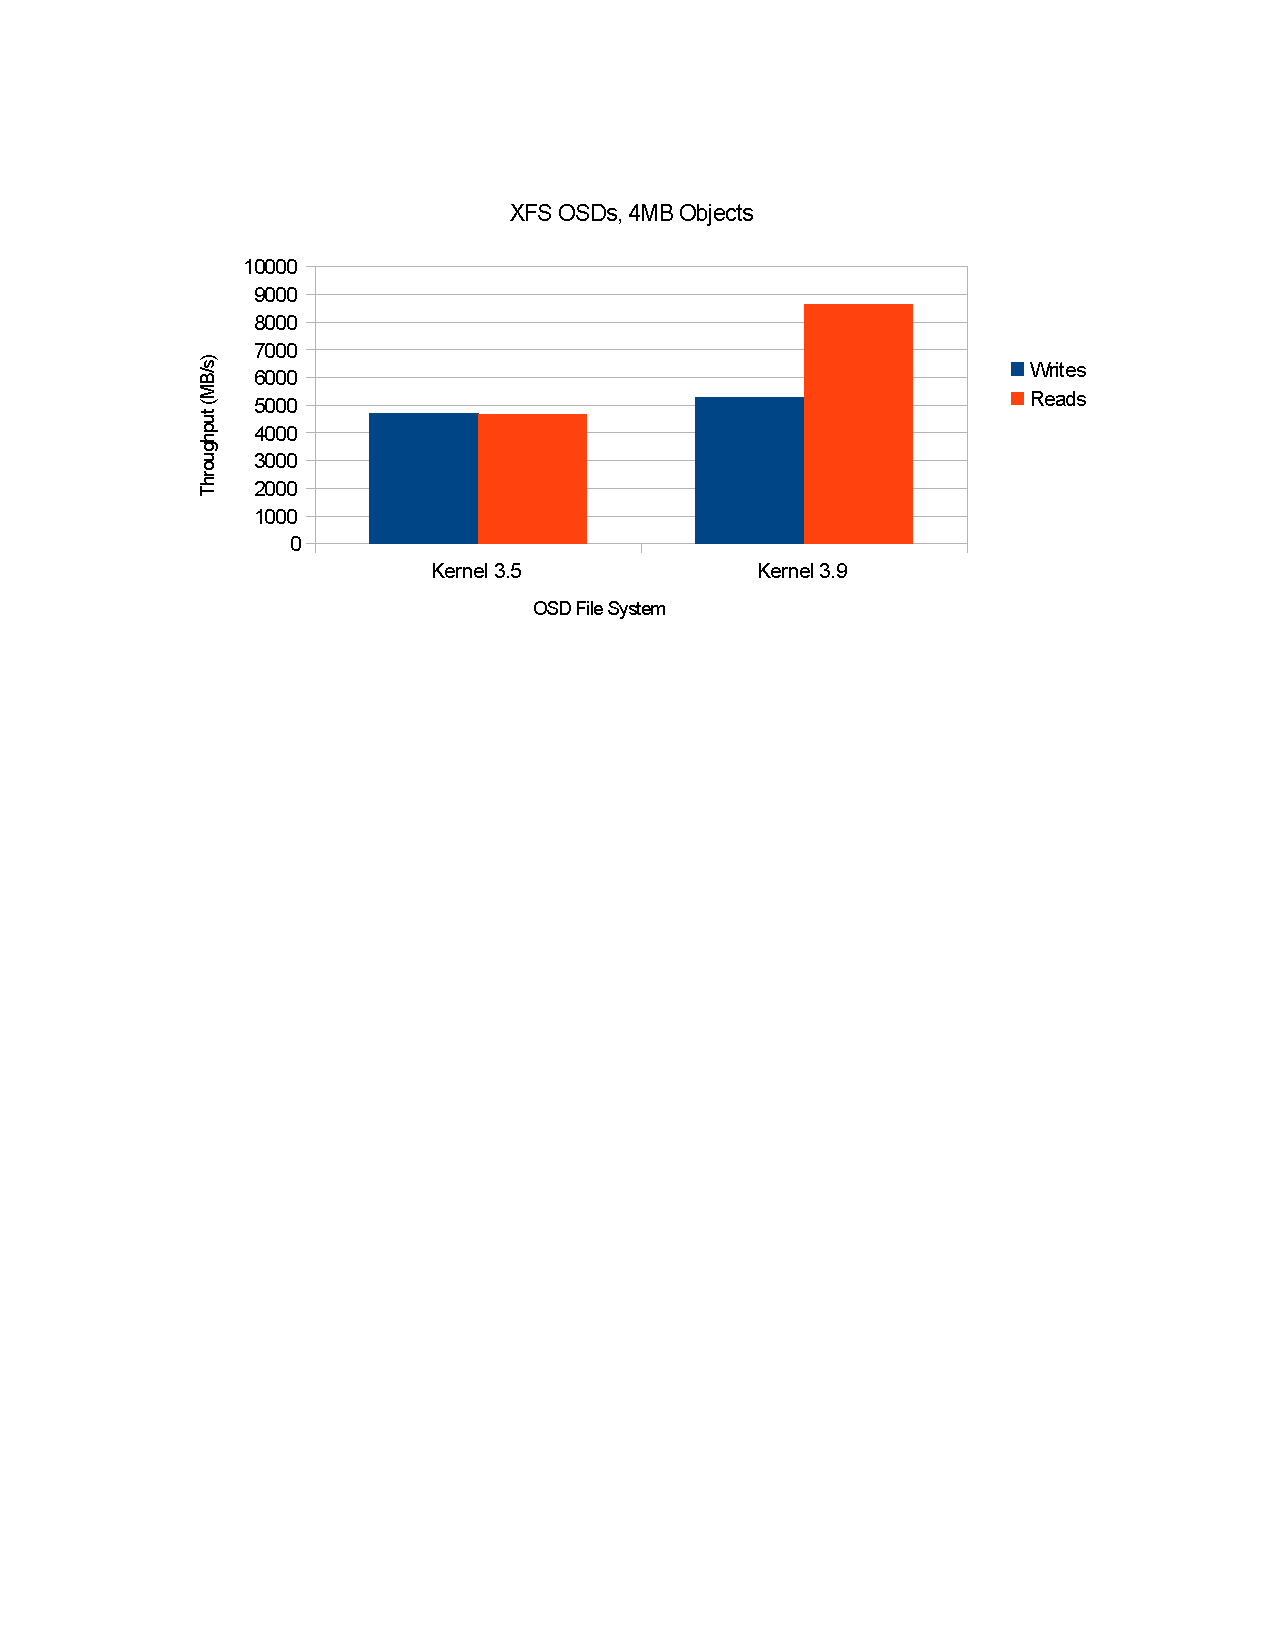
\includegraphics[width=4in]{rados-kernel-35vs39}
\caption{RADOS bench: Kernel 3.5 vs. 3.9}
\label{fig:rados-kernel}
\end{figure}



With the kernel changes writes performance improved slightly, while read
performance improved dramatically.  In addition to the kernel change, Sage Weil
suggested increasing the amount of read ahead being performed by the CephFS
kernel client:

\begin{Verbatim}[samepage=true]
mount -t ceph 10.37.248.43:6789:/ /mnt/ceph -o
   name=admin,nocrc,readdir_max_bytes=4104304,readdir_max_entries=8192
\end{Verbatim}


\begin{figure}[htb]
\centering
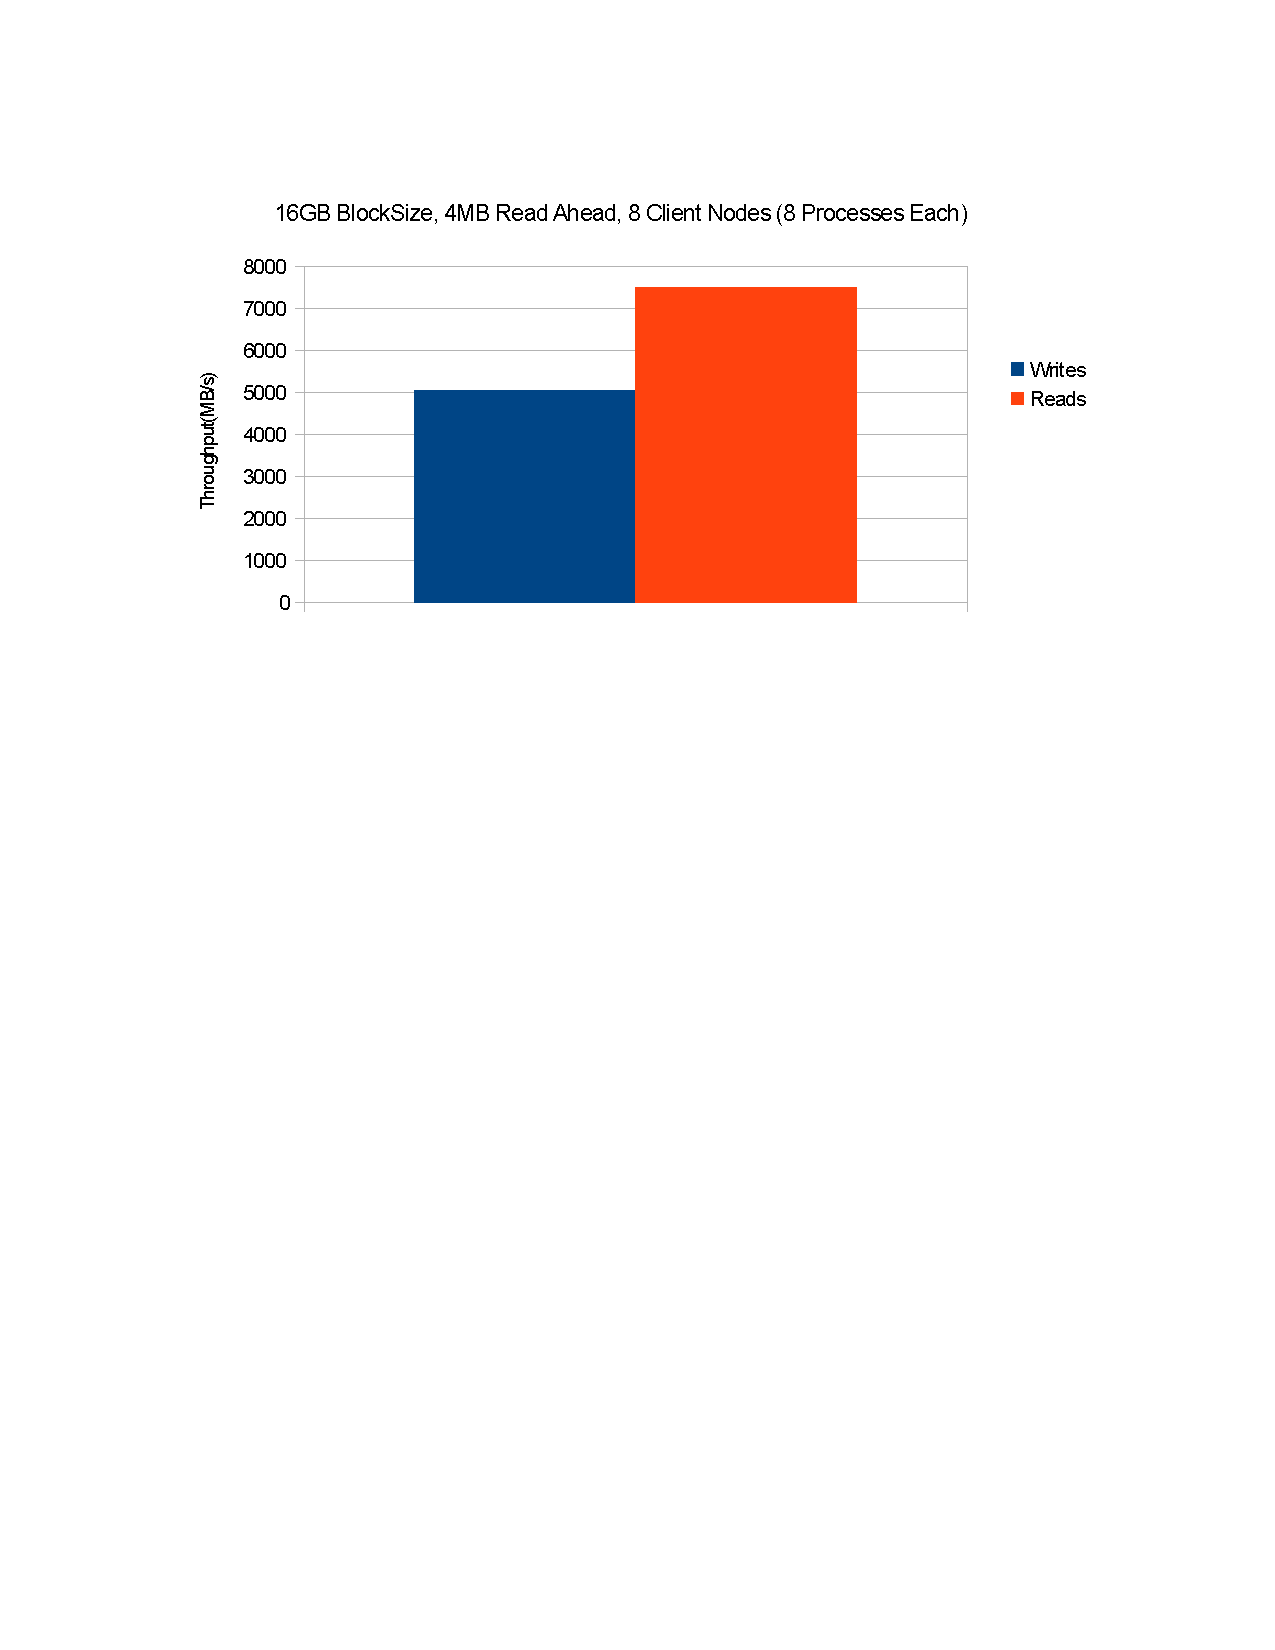
\includegraphics[width=4in]{ior-kernel-39}
\caption{Kernel changes to 3.9, IOR with 4MB transfer size}
\label{fig:ior-kernel-39}
\end{figure}


By installing a new kernel, increasing read ahead, and increasing the number of
client IOR processes, we were able to achieve a very satisfactory result on this
test run.


\subsection{Repeating IOR Scaling Test}

As before, we ran IOR scaling test with two cases: transfer size 4K and 4M.
These results are illustrated in Figure~\ref{fig:ior-064}. As expected, we are
seeing a much improved picture of read and write performance, very much in
line with RADOS bench performance.

\begin{figure}[htb]
\centering
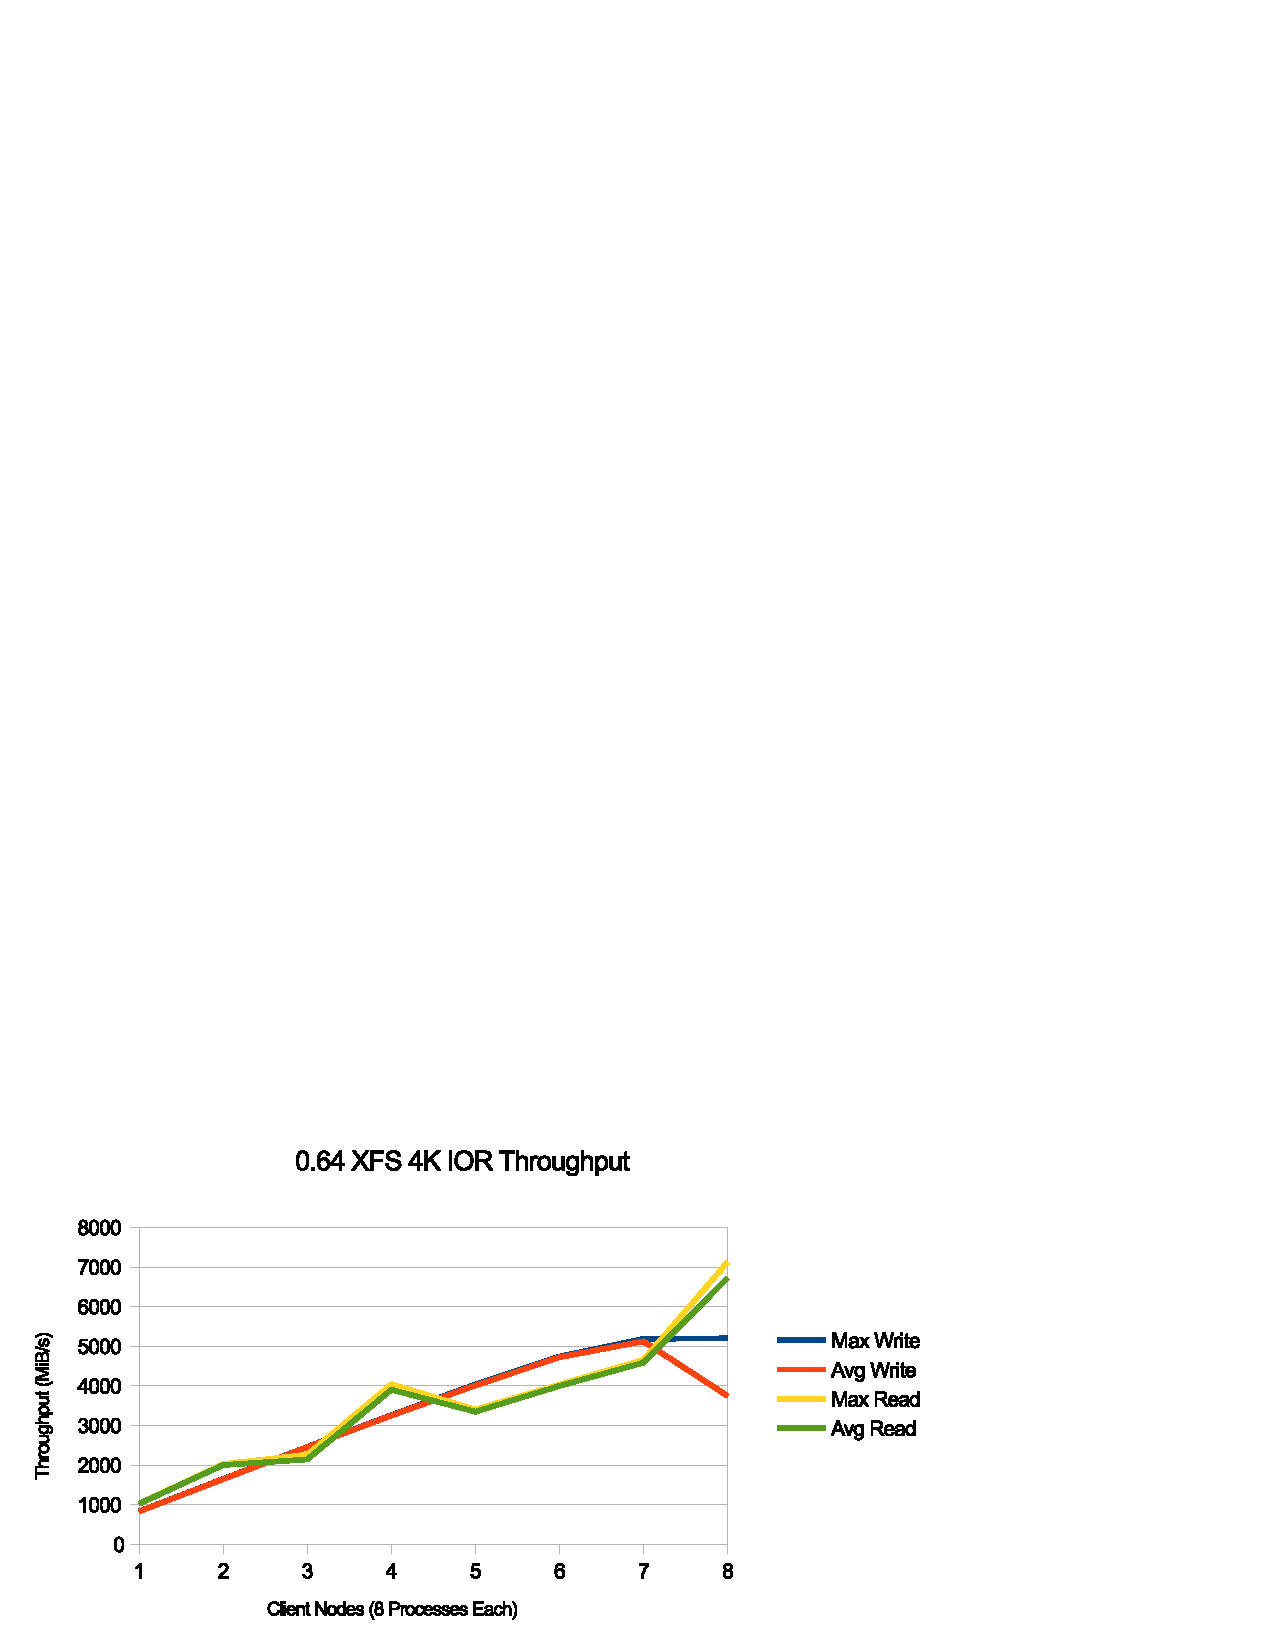
\includegraphics[width=5in]{ior-064-4k}
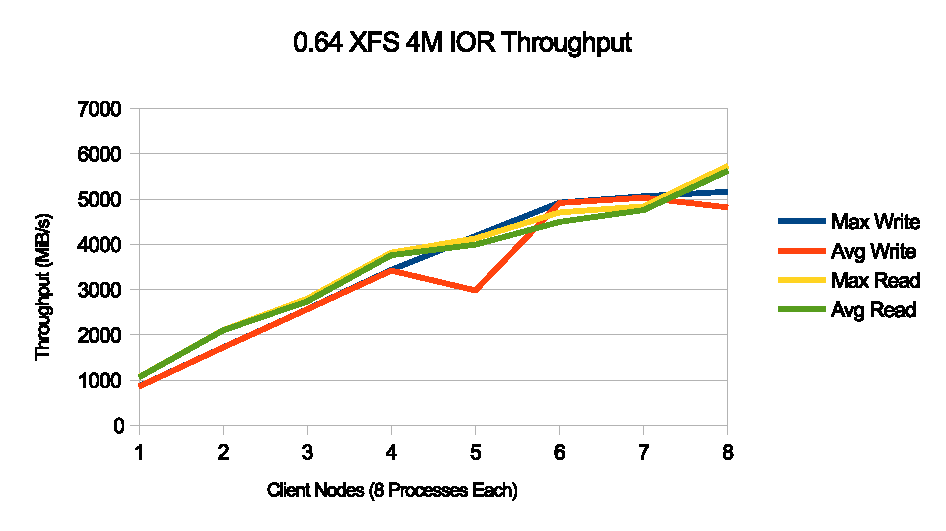
\includegraphics[width=5in]{ior-064-4m}
\caption{IOR Scaling Test: 4KB and 4MB transfer size}
\label{fig:ior-064}
\end{figure}

We observe that a couple of places where the average write throughput is quite a
bit lower than the max.  This behavior was observed during other tests as well,
indicating that we may have periods of time where write throughput is
temporarily degrading.  Despite these issues, performance general seems to be
improving as the number of clients increases.  Writes seem to be topping out at
around 5.2GB/s (which is roughly what we would expect).  Reads seem to be
topping out anywhere from 5.6-7GB/s, however it is unclear if read performance
would continue scaling with more clients and get closer to the 8GB/s+ numbers we
saw with RADOS Bench.


\section{Metadata Performance}


In our particular setup, we have only one metadata server (MDS)
configured. Therefore, this is not a scalability test on the performance of
clustered MDS, which would be very interesting and might as well come later.
Instead, we focus on a single MDS, multiple clients (up to 8) and see how it
scales. The particular parameters we use for testing are:

\begin{itemize}
\item \verb!-w 1048576 -y!: for each created file, we write 1 MB data and
perform sync after it. This is a more realistic use case scenario than just
open, close and removal.

\item \verb!-n 1000!: this is per client file \textit{and} directories. For 8
clients, the number of files and directories is 8,000. Since we didn't specify
either \verb!-D! or \verb!-F!, so this is a mixture of both.

\item \verb!-d /mnt/cephfs/tmp!: we do specify a directory, but unlike under
Lustre file system, where you can have single client multiple mounts (for
increasing workload per client), here we just give the test an explicit home.

\item \verb!-u!: without this option, we are exercising shared directory; with
this option, we are exercising unique directories.

\end{itemize}

Each test iterates 5 times and we are showing the max. 
We summarize the results as follows:

%Figure~\ref{fig:mdtest1c} is meant to give an overview on the trending of each
%directory (prefixed with d) and file (prefixed with f) operations, against the
%number of clients. Due to the scale difference, it doesn't convey the
%magnitude of lower numbers. 

\begin{itemize}

\item Within a single sharing mode (either shared or unique directory), the
directory stat and file stat, as well as file read exhibit strong linear
scaling property. 

\item While the other operations seems unaffected or flat by the number of
clients, it is not so if we zoom in, see \ref{fig:mdtest-fcreate} and
\ref{fig:mdtest-dcreate}:  as number of clients increases, we observed the
contention for shared directory. The performance degradation amount to 50\% or
more.

\item Though the same saturation or degradation trend is not observed for file
creation, it is likely due to we have not put enough of workload stress on MDS.

\end{itemize}


\begin{figure}[htb]
\centering
%% -- 1st figure
\begin{minipage}[t]{0.5\linewidth}
\centering
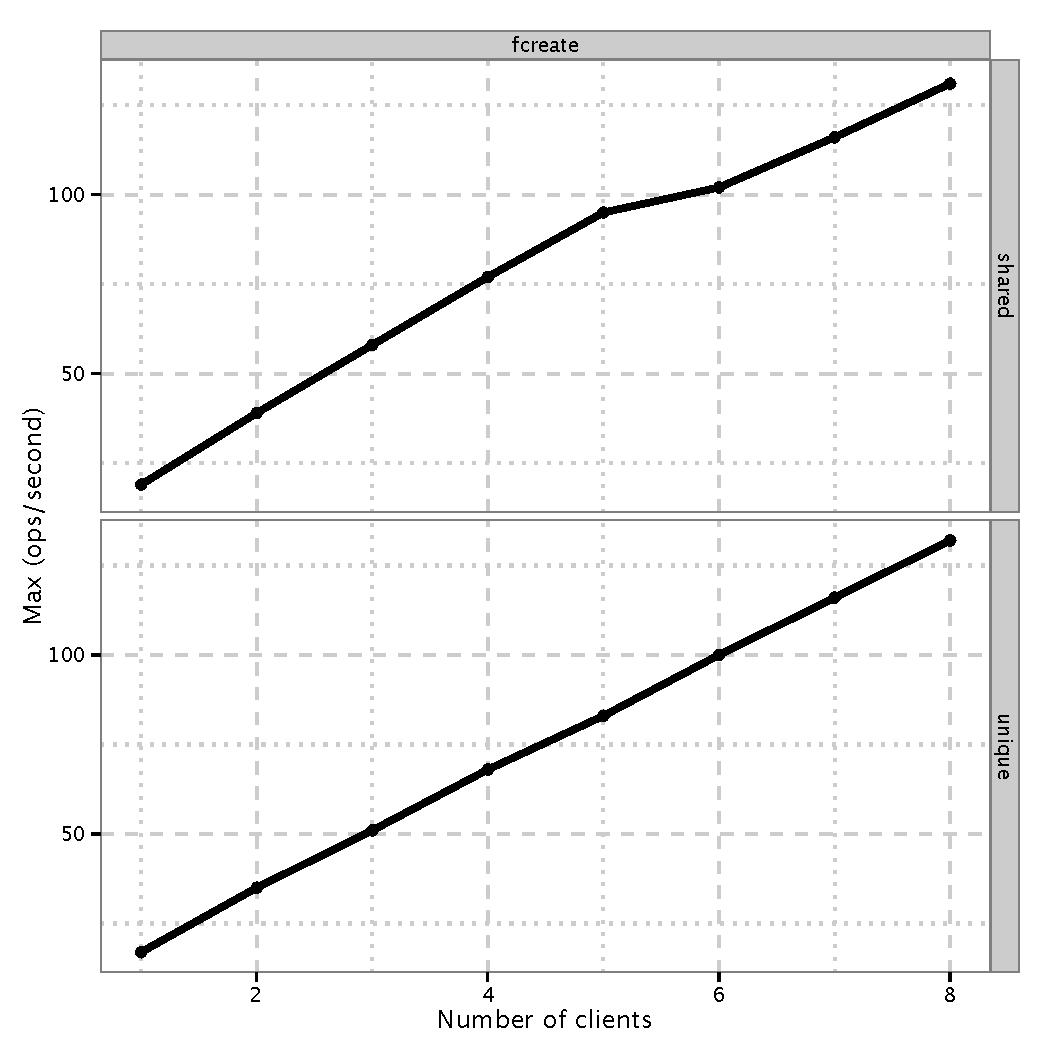
\includegraphics[width=3in]{data/mdtest-fcreate}
\caption{file creation vs.  \# of clients}
\label{fig:mdtest-fcreate}
\end{minipage}%
\begin{minipage}[t]{0.5\linewidth}
\centering
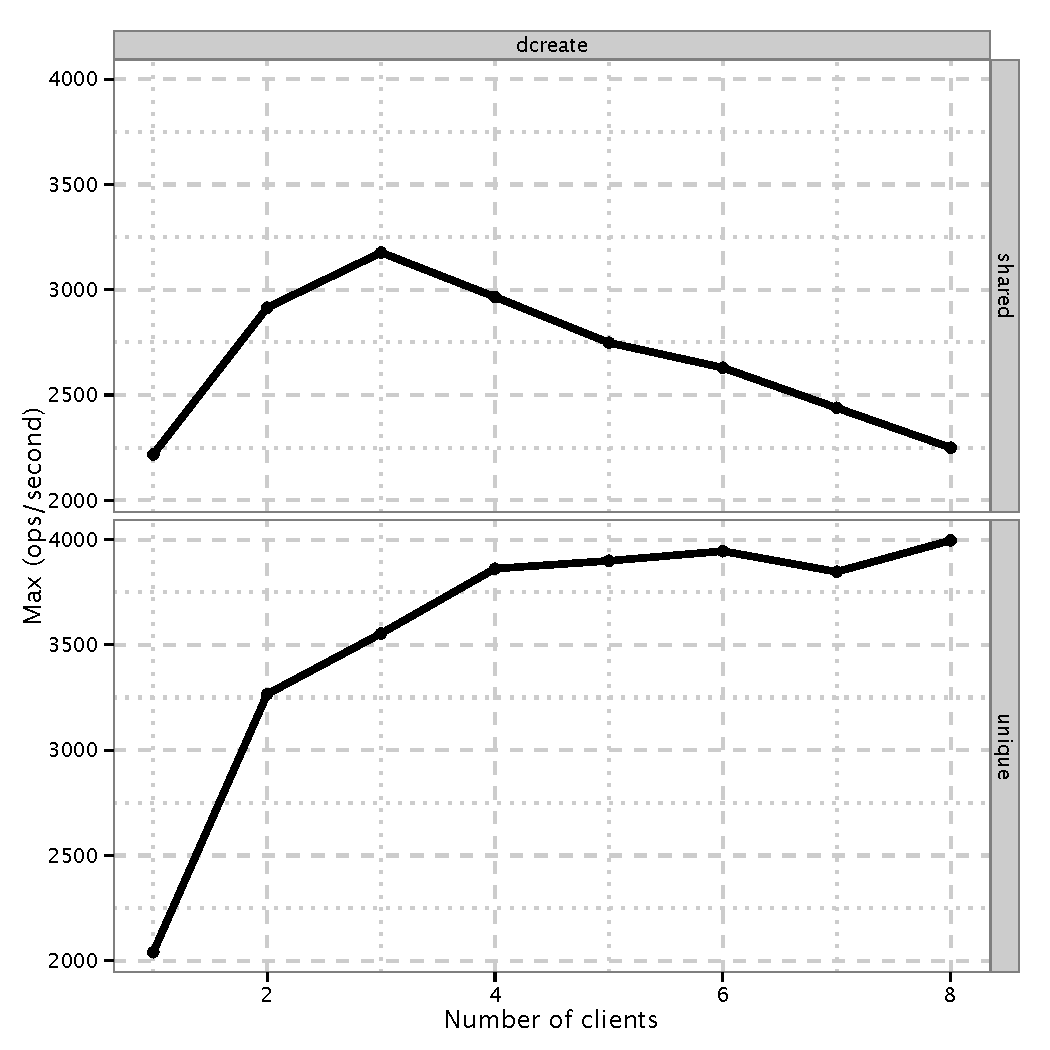
\includegraphics[width=3in]{data/mdtest-dcreate}
\caption{directory creation vs. \# of clients}
\label{fig:mdtest-dcreate}
\end{minipage}%
\end{figure}


\section{Observations and Conclusions}

This is preliminary observations from mostly performance perspective:

\begin{itemize}

  \item Ceph is built on the assumption that the underlying hardware components
  is unreliable, with little or no redundancy and failure detection capability.
  This is not the case in this leadership computing facilities. We have disabled
  replication for pools, but this will take a toll somewhere in the processing
  and we don't know if this is significant.

  \item Ceph do \textbf{metadata + data} journaling, which is fine for host
  system that has locally attached disk. However, this presents a problem in DDN
  SFA10-like hardware, where the backend LUNs are exposed as block device
  through SRP over IB. The journaling write would requires double bandwidth
  compare to Lustre-like metadata only journaling mechanism. For Ceph to anything
  viable in this facility, there has to be a solution for this.

  \item Ceph is observed to have consist results and linear scalability at the
  RADOS level. However, it broke down at the file system level with synthetic
  benchmark suite such as IOR. We have experience large performance swings
  during different runs, very low read performance when transfer size is small,
  and IO errors tend to happen when system is under stress (more clients and
  large transfer size). These are not particularly reproducible results, but it
  suggests the level of maturity still have a long way to go.
  
\end{itemize}

\section*{Appendix A - CephFS Final Mount Command}
\addcontentsline{toc}{section}{Appendix A - CephFS Final Mount}

\begin{Verbatim}
mount -t ceph 10.37.248.43:6789:/ /mnt/ceph -o
      name=admin,nocrc,readdir_max_bytes=4104304,readdir_max_entries=8192
\end{Verbatim}


\section*{Appendix B - OSD File System Options}
\addcontentsline{toc}{section}{Appendix B - OSD File System Options}

\input{osd_fs.txt}

\section*{Appendix C - CRUSH Map}
\addcontentsline{toc}{section}{Appendix C - CRUSH map}

This crush map is just an example of full OSD mapping. As we create and
re-create different testbed with different OSD configurations, the map will
change accordingly.

\input{crush.txt}


\section*{Appendix D - Final ceph.conf}
\addcontentsline{toc}{section}{Appendix D - Final ceph.conf}

\input{ceph-short.txt}


\end{document}
